%%%%% CHOOSE PAGE LAYOUT
% The most common choices should be below.  You can also do other things, like replacing "a4paper" with "letterpaper", etc.

% This one will format for two-sided binding (ie left and right pages have mirror margins; blank pages inserted where needed):
%\documentclass[a4paper,twoside]{ociamthesis}
% This one will format for one-sided binding (ie left margin > right margin; no extra blank pages):
%\documentclass[a4paper]{ociamthesis}
% This one will format for PDF output (ie equal margins, no extra blank pages):
\documentclass[a4paper,nobind]{ociamthesis} 
\usepackage{pgfplots}
\pgfplotsset{compat=newest}
\usepackage{tikz}
\usepackage{siunitx}

%%%%% SELECT YOUR DRAFT OPTIONS
% Three options going on here; use in any combination.  But remember to turn the first two off before
% generating a PDF to send to the printer!

% This adds a "DRAFT" footer to every normal page.  (The first page of each chapter is not a "normal" page.)
\fancyfoot[C]{\emph{DRAFT Printed on \today}}  

% This highlights (in blue) corrections marked with (for words) \mccorrect{blah} or (for whole
% paragraphs) \begin{mccorrection} . . . \end{mccorrection}.  This can be useful for sending a PDF of
% your corrected thesis to your examiners for review.  Turn it off, and the blue disappears.
\correctionstrue


%%%%% BIBLIOGRAPHY SETUP
% Note that your bibliography will require some tweaking depending on your department, preferred format, etc.
% The options included below are just very basic "sciencey" and "humanitiesey" options to get started.
% If you've not used LaTeX before, I recommend reading a little about biblatex/biber and getting started with it.
% If you're already a LaTeX pro and are used to natbib or something, modify as necessary.
% Either way, you'll have to choose and configure an appropriate bibliography format...

% The science-type option: numerical in-text citation with references in order of appearance.
\usepackage[style=numeric-comp, sorting=none, backend=biber, doi=false, isbn=false]{biblatex}
\newcommand*{\bibtitle}{References}

% The humanities-type option: author-year in-text citation with an alphabetical works cited.
%\usepackage[style=authoryear, sorting=nyt, backend=biber, maxcitenames=2, useprefix, doi=false, isbn=false]{biblatex}
%\newcommand*{\bibtitle}{Works Cited}

% This makes the bibliography left-aligned (not 'justified') and slightly smaller font.
\renewcommand*{\bibfont}{\raggedright\small}

% Change this to the name of your .bib file (usually exported from a citation manager like Zotero or EndNote).
\addbibresource{references.bib}


% Uncomment this if you want equation numbers per section (2.3.12), instead of per chapter (2.18):
%\numberwithin{equation}{subsection}


%%%%% THESIS / TITLE PAGE INFORMATION
\title{Experimental apparatus for universal spin-motion control in trapped multi-ion crystals}
\author{Donovan Webb}
\college{St Peter's College}

\degree{Doctor of Philosophy}
% Term and year of submission, or date if your board requires (eg most masters)
\degreedate{Trinity 2025}


%%%%% YOUR OWN PERSONAL MACROS
% This is a good place to dump your own LaTeX macros as they come up.

% To make text superscripts shortcuts
	\renewcommand{\th}{\textsuperscript{th}} % ex: I won 4\th place
	\newcommand{\nd}{\textsuperscript{nd}}
	\renewcommand{\st}{\textsuperscript{st}}
	\newcommand{\rd}{\textsuperscript{rd}}
	\newcommand{\ca}{\textsuperscript{40}Ca\textsuperscript{+}}

%%%%% THE ACTUAL DOCUMENT STARTS HERE
\begin{document}


%%%%% CHOOSE YOUR LINE SPACING HERE
% This is the official option.  Use it for your submission copy and library copy:
\setlength{\textbaselineskip}{22pt plus2pt}
% This is closer spacing (about 1.5-spaced) that you might prefer for your personal copies:
%\setlength{\textbaselineskip}{18pt plus2pt minus1pt}

% You can set the spacing here for the roman-numbered pages (acknowledgements, table of contents, etc.)
\setlength{\frontmatterbaselineskip}{17pt plus1pt minus1pt}

% Leave this line alone; it gets things started for the real document.
\setlength{\baselineskip}{\textbaselineskip}


%%%%% CHOOSE YOUR SECTION NUMBERING DEPTH HERE
% You have two choices.  First, how far down are sections numbered?  (Below that, they're named but
% don't get numbers.)  Second, what level of section appears in the table of contents?  These don't have
% to match: you can have numbered sections that don't show up in the ToC, or unnumbered sections that
% do.  Throughout, 0 = chapter; 1 = section; 2 = subsection; 3 = subsubsection, 4 = paragraph...

% The level that gets a number:
\setcounter{secnumdepth}{2}
% The level that shows up in the ToC:
\setcounter{tocdepth}{3}


%%%%% ABSTRACT SEPARATE
% This is used to create the separate, one-page abstract that you are required to hand into the Exam
% Schools.  You can comment it out to generate a PDF for printing or whatnot.
%\begin{abstractseparate}
%    \input{text/abstract} % Create an abstract.tex file in the 'text' folder for your abstract.
%\end{abstractseparate}


% JEM: Pages are roman numbered from here, though page numbers are invisible until ToC.  This is in
% keeping with most typesetting conventions.
\begin{romanpages}

% JEM: By default, this template uses the traditional Oxford "Belt Crest". Un-comment the following
% line to use the newer, "Blue Square" logo:
% \renewcommand{\crest}{{
\includegraphics[width=4.2cm, height=4.2cm]{figures/newlogo.pdf}}}

% Title page is created here
\maketitle

%%%%% DEDICATION -- If you'd like one, un-comment the following.
%\begin{dedication}
%This thesis is dedicated to\\
%someone\\
%for some special reason\\
%\end{dedication}

%%%%% ACKNOWLEDGEMENTS -- Nothing to do here except comment out if you don't want it.
%\begin{acknowledgements}
%    \input{text/acknowledgements}
%\end{acknowledgements}

%%%%% ABSTRACT -- Nothing to do here except comment out if you don't want it.
%\begin{abstract}
%    \input{text/abstract}
%\end{abstract}

%%%%% MINI TABLES
% This lays the groundwork for per-chapter, mini tables of contents.  Comment the following line
% (and remove \minitoc from the chapter files) if you don't want this.  Un-comment either of the
% next two lines if you want a per-chapter list of figures or tables.
\dominitoc % include a mini table of contents
%\dominilof  % include a mini list of figures
%\dominilot  % include a mini list of tables

% This aligns the bottom of the text of each page.  It generally makes things look better.
\flushbottom

% This is where the whole-document ToC appears:
\tableofcontents

%\listoffigures
	%\mtcaddchapter
% \mtcaddchapter is needed when adding a non-chapter (but chapter-like) entity to avoid confusing minitoc

% Uncomment to generate a list of tables:
%\listoftables
%	\mtcaddchapter


% The Roman pages, like the Roman Empire, must come to its inevitable close.
\end{romanpages}


%%%%% CHAPTERS
% Add or remove any chapters you'd like here, by file name (excluding '.tex'):
\flushbottom
\section{Motivation}
% Main points:
    % High overview of work.
    % Describe that have spent two years building this system.
    % Building a system with spin and motion control.
    % List of unique requirements for the system
        % Motional control
        % Single addressing
        % Standing waves
    % Here characterisation
    % But we want to use this experiment for...
        % E.g. Feynman diagram simulation
        % Here I would like to briefly describe the next steps in the project, as well
        % as the future experiments we want to demonstrate.
        % Discussion of single addressing could be here.

    The following chapter details the characterisation work performed during the
    commisioning of a new ion trap apparatus. Over the past two years, my
    colleagues and I have been constructing this system, which is now
    approaching readiness for our desired experiments. In this
    \textit{Motivation} section, I will provide a high-level overview of the
    physics we want to explore, state the unique aspects of the apparatus that
    enable these experiments, and finally, give a timeline for planned future
    work. The complexity of our system neccesitates collaboration, and so I
    would like to acknowledge the rest of the \emph{FastGates} team, for their
    extensive contributions to bringing the system online. \\

    There are two research directions that we are pursuing with this apparatus.
    Both involve the study and interplay between the ``spin'' electronic degree
    of freedom and the motion of the ion which we describe by a quantum harmonic
    oscillator.\\
    The first is the demonstration of fast and high-fidelity two-qubit
    entangling gates between trapped ions. High fidelity entangling gates are
    critical for developing a quantum computer which can perform useful
    calculations with high success probability~\cite{steane2003overhead}. Gate errors associated with
    decoherence of the quantum state are often dominated by incoherent
    processes, such as spontaneous emission, or interactions between the qubit
    and the environment~\cite{wineland1998experimental}. These errors accumulate with time, and so may be
    mitigated by increasing the algorithm ``clock-speed'', hence our desire for
    fast entanglement~\cite{steane2000speed,schafer2018fast}. Typically in ion traps, local two-qubit gates are
    performed via the ion's shared motion, which may be excited by interaction
    with a laser~\cite{cirac1995quantum, sorensen2000entanglement}. As the effective gate frequency approaches that of the
    frequency separation of the motional modes, the dynamics between spin and
    motion become complicated by multiple simultaneous mode excitations~\cite{schafer2018fast}. Our
    apparatus is designed to provide the required laser intensities and mode
    frequencies such that we can explore this regime, and demonstrate the
    required control to tame these multiple mode excitations and perform
    high-fidelity entangling gates.\\
    The second direction is the use of the motion of the ion directly as a
    quantum resource~\cite{liu2024hybrid,chen2021quantum}. This falls into the continuous variable quantum computing
    paradigm (CVQC), where instead of discrete qubits, the quantum state is
    described by bosonic ``qumodes''~\cite{lloyd1999quantum}. CVQC reduces the
    technical overhead of scaling discrete systems, as larger Hilbert spaces are
    easily accessed due to the many level nature of the individual qumodes.
    We want to demonstrate a
    universal set of gates for CVQC, which includes, single-mode Gaussian and
    non-Gaussian gates (demonstrated in~\cite{bazavan2024squeezing}), and two-mode entangling gates. Further, we want to demonstrate the ability to simultaneously leverage both
    bosonic and spin degrees of freedom of our ions to efficiently encode
    problems in the full hybrid system we have access to~\cite{varona2024towards, brenner2024factoring}. Our apparatus has both
    precise motional control and stability through our trap choice, and the
    selective addressing system that is required when interacting with many-ion
    chains.\\
    
    Details of the apparatus are presented in the Appendices. Summarised here are the unique aspects enabling the desired experiments:
    \begin{itemize}
    \item \textbf{High laser intensities:} The system is designed to provide
        high laser intensities, which are required to drive fast entangling
        gates. This is achieved through the use of a 5~W Ti:Sapph system (section~\ref{sec:Narrow Line Width 729 Laser}) and
        two high numerical aperture (NA = 0.6) objectives (section~\ref{sec:Vacuum System}).
    \item \textbf{Single ion addressing:} Using crossed acousto-optic
        deflectors, we can selectively address individual ions in a multi-ion chain (section~\ref{sec:Single Addressing System}).
        This enables fast entangling gates between ions in a long
        chain, and the ability to perform motional interactions on selected modes.
    \item \textbf{Standing wave addressing:} The system is designed to provide
        standing optical waves at the ion position. Standing waves are required for
        some fast gate schemes~\cite{saner2023breaking}. 
    \item \textbf{Motional control:} The Paul trap used in the system, produced
        by \emph{National Physical Laboratory} in the UK, has low heating rates (section~\ref{sec:Heating}),
        deep trapping potentials relative to surface style ion traps, and flexible
        control over DC confinement (section~\ref{sec:The Ion Trap}). These features ensure that we have modes
        with long coherence times (section~\ref{sec:Motional Mode Stability}), making them suitable for encoding quantum
        information.
    \end{itemize}

    Here, the characterisation of the spin qubits is in the context of discrete
    variable quantum computing. We are interested in the fidelity of qubit
    state-preparation, measurement (sections~\ref{sec:Stateprep,sec:Measurement}), single- (section~\ref{sec:Single Qubit Gates}) and two-qubit gates (section~\ref{sec:Two-Qubit Entangling Gates}). These
    individual elements comprise longer circuits, and so all contribute to the
    overall fidelity of any chosen algorithm.\\
    The motional characterisation is currently focused on the stability of the
    modes (section~\ref{sec:Motional Mode Stability}), and the ability to perform spin-dependent forces, SDFs (section~\ref{sec:Spin-Dependent Forces}). SDFs are the
    base interaction on which many of the desired CVQC gates are
    comprised~\cite{sutherland2021universal}, and so these must be well
    characterised and understood in our system.\\

    To push the system forwards, in the next 6~months, we will focus on
    commisioning the single addressing system, and on demonstrating squeezing of
    the motional state of the ion.\\
    As described above, the single addressing system is a critical component for
    many of our planned experiments. Section~\ref{sec:Single Addressing System},
    and~\cite{oevergaard2024limiting} describe the system in detail. The next
    immediate steps are to align the constructed optical system to the ion
    chain, and to implement the logical and RF control system required to drive
    the acousto-optic deflectors. Once this is complete, we will characterise
    the cross-talk of the system by performing single addressing of ions in a
    chain and measuring spin populations. We will then be able to demonstrate
    fast entangling gates between ions in a chain, and the ability to perform
    motional interactions on selected modes.\\
    Squeezing of the motional mode via the method outlined
    in~\cite{sutherland2021universal}, is a significant step towards
    demonstrating the universal set of gates for CVQC. This is due to
    the constituent interactions of the effective squeezing gate (two SDFs), are
    the same interactions needed for trisqueezing~\cite{braunstein1987generalised, bazavan2024squeezing} --- a non-Gaussian gate, and
    for two-mode squeezing~\cite{lvovsky2015squeezed} --- an entangling gate. Furthermore, once we have
    demonstrated generating squeezing characteristic functions, there is a clear
    path to experimentally demonstrating the extraction of Feynman diagram terms
    with the hybrid system being used as a quantum
    simulator~\cite{varona2024towards}.\\

\chapter{Experimental Characterisation}
\label{ch:Characterisation}
\minitoc

    Before we can proceed with our planned experiments involving the motion and
    spin of the atoms, the apparatus must be characterised. This characterisation
    serves two purposes: it allows us to benchmark the performance of our system
    against state-of-the-art results, and it reveals any current limitations
    that must be addressed before we can successfully carry out the experiments.\\
    As discussed above, we are interested in two paradigms: discrete variable quantum computing (DVQC), that concerns the manipulation of qubits (or spins), and continuous variable quantum computing (CVQC), that concerns the manipulation of qumodes (or harmonic motion).\\
    For DVQC, we must have access to the following elementary operations:
    \begin{itemize}
        \item Qubit state preparation, here via optically pumping the electronic state of the ion into one sublevel of the $4S_{1/2}$ manifold --- the lower level of our qubit, section~\ref{sec:Stateprep}.
        \item Measurement of the qubit state, here via state-dependent fluorescence, section~\ref{sec:Measurement}.
        \item Single qubit rotations, here via interaction with the 729-nm laser, section~\ref{sec:Single Qubit Gates}
        \item Two qubit entangling-gates, here via spin-dependent forces (SDFs), using the 729-nm laser and the motional modes of the ion, section~\ref{sec:Two-Qubit Entangling Gates}.
    \end{itemize}
     For CVQC, we need:
    \begin{itemize}
        \item Motional state preparation, here via Doppler cooling and sideband cooling, section~\ref{sec:Cooling}.
        \item Measurement of the motional state, which is not yet implemented on our system but will follow~\cite{fluhmann2020direct}.
        \item Single and two qumode gates, which are also not yet implemented, but will utilise SDFs following~\cite{sutherland2021universal}, section~\ref{sec:Spin-Dependent Forces}.
    \end{itemize}
    We split this chapter into interactions involving only the spin, then those focussed only on the motion, and finally we describe spin-motion interactions.
    First, however, we describe the ion, its level structure, and the relevant lasers to manipulate its state.


\section{The Ion}
\label{sec:Transitions}
% Main points:
    % All visible motional modes on large detuning scan at $5$~G. 
    % Can compare when have all quadrupole transitions available or when we selectively omit transitions via polarisation.
% Pre reqs:
    % 5 G field
    \begin{figure}[ht]
        \begin{center}
        \noindent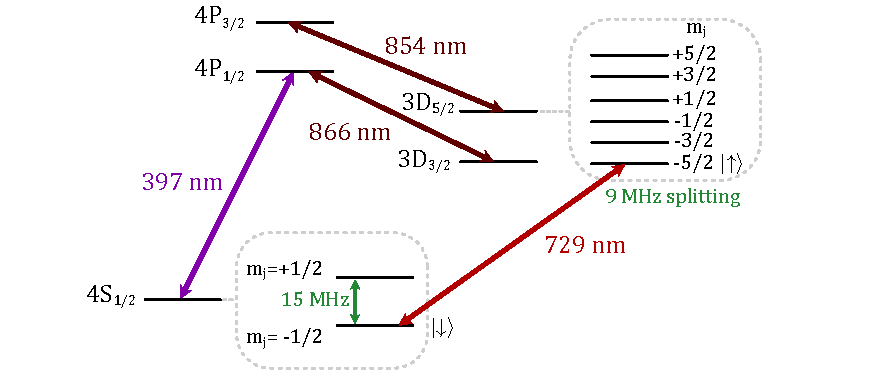
\includegraphics[width=\linewidth]{figures/pdf_figure/ion.pdf}
        \end{center}
        \caption{
        Electronic energy levels of \textsuperscript{40}Ca\textsuperscript{+},
        which will be used in this thesis. The levels are
        split by the Zeeman effect due to a $5.4$~G external magnetic field (they are shown explicitely only for the qubit manifolds). The
        transitions marked are required for cooling and control over the
        ion. The chosen qubit levels are labelled with $\ket{\downarrow}$, $\ket{\uparrow}$.
        }

    \label{fig:ion}
    \end{figure}

    \begin{figure}
        \vspace*{-0.5cm}
        \begin{center}
        \noindent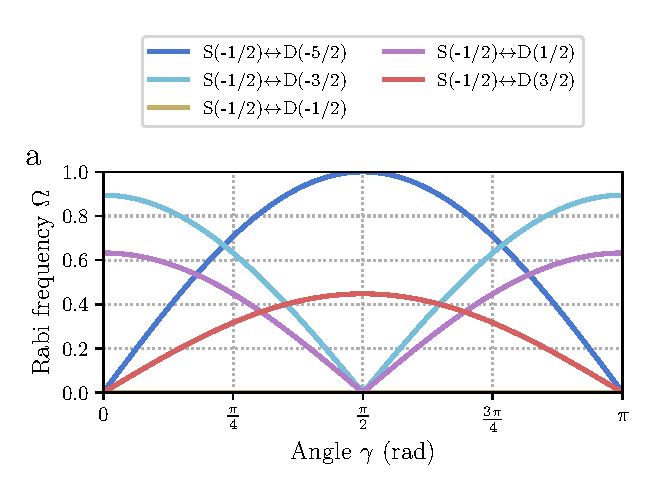
\includegraphics[width=0.65\linewidth]{
            figures/pdf_figure/qp_gamma.pdf
            }
        \vspace*{-0.5cm}
        \noindent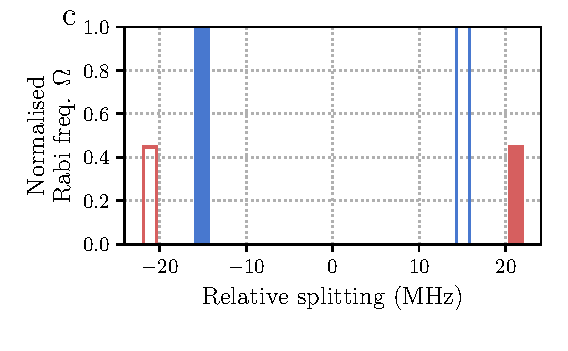
\includegraphics[width=0.65\linewidth]{
            figures/pdf_figure/qp_transition_spectrum_0.50.pdf
            }
        \vspace*{-0.5cm}
        \noindent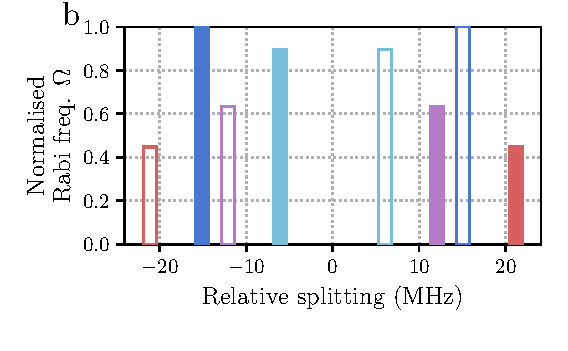
\includegraphics[width=0.65\linewidth]{
            figures/pdf_figure/qp_transition_spectrum_0.25.pdf
            }
        \end{center}
        \vspace*{-0.5cm}
        \caption{
            Normalised quadrupole Rabi frequencies, $\Omega$, and frequency splittings for the $4S_{1/2} \leftrightarrow 3D_{5/2}$ Zeeman sublevels in \ca. Solid bars correspond to transitions with lower state $\ket{4S_{1/2},~m_j = -1/2}$, while open bars correspond to transitions with lower state $\ket{4S_{1/2},~m_j = +1/2}$.
            \textbf{a)} Relative Rabi frequencies as angle $\gamma$ between the polarisation vector and the magnetic field is varied. The k-vector of the light is assumed to be perpendicular to the B-field.
            \textbf{b)} Relative frequency splittings and strengths when $\gamma = \pi/2$. This is the polarisation chosen for the current and future experiments to reduce the number of transitions which can cause off-resonant interactions when the qubit defined by $\ket{4S_{1/2},~m_j = -1/2} \leftrightarrow \ket{3D_{5/2},~m_j = -5/2}$ is used.
            \textbf{c)} Relative frequency splittings and strengths when $\gamma = \pi/4$. At this angle, all transitions are accessible apart from those with $\Delta m_j = 0$. This is the polarisation chosen for our initial experiments to allow access to all transitions for characterisation.
            }
        \label{fig:quadrupole}
    \end{figure}

    The \ca ion has a rich level structure, shown in figure~\ref{fig:ion}, with many accessible quadrupole transitions $4S_{1/2}\leftrightarrow 3D_{5/2}$. The quadrupole transition is ideal for use as a qubit due to the long-lived metastable level ($\tau=1.1$~\unit{\s})~\cite{barton2000measurement}, and the ability to optically couple the transition via a laser. As mentioned in section~\ref{sec:Narrow Line Width 729 Laser}, the 729-nm beam is used for this purpose. By selecting the appropriate frequency of the 729-nm beam, qubit operations such as state preparation (section~\ref{sec:Stateprep}) and single qubit gates (section~\ref{sec:Single Qubit Gates}) may be driven, or by setting the detuning such that a motional sideband is near resonance, to couple the spin and motional degrees of freedom (section~\ref{sec:Spin-Dependent Forces}). Here, we discuss which quadrupole transitions are used, and the rationale behind their choice.\\ 
    Zeeman splitting of the $4S_{1/2}$ and $3D_{5/2}$ states leads to 2 and 6
    non-degenerate sublevels, respectively. Due to the magnetic field strength of 5.4~G (section~\ref{sec:Magnetic Field}),
    the $S$-levels are split by $\sim$15~\unit{\MHz}, and the $D$-levels by $\sim$9~\unit{\MHz}.
    This splitting is considerably larger than both the natural linewidth of the
    729-nm transition ($\sim$\unit{\Hz}), and the Ti:Sapph laser linewidth (<1~\unit{\kHz}), meaning the transitions can be 
    selectively addressed by frequency tuning of the laser. There is some freedom in choosing which of these 10 possible (with $\Delta m_j \leq 2$) quadrupole transitions we define as our qubit. Each transition has a varying coupling strength, here denoted by the relative Rabi frequency, $\Omega$, depending on the polarisation and $k$-vector of the interacting light with respect to the B-field axis. The desired criteria for qubit and polarisation choice are as follows:
    \begin{itemize}
    \item Access to a closed-cycle transition for sideband cooling, (for details on this, see section~\ref{sec:Cooling}). Closed-cycle here means $\ket{4S_{1/2},~m_j = -1/2} \rightarrow \ket{3D_{5/2}} \rightarrow \ket{4P_{3/2},~m_j = -3/2} \rightarrow \ket{4S_{1/2},~m_j = -1/2}$.
    \item The qubit transition needs a large quadrupole matrix element, leading to a high Rabi frequency, $\Omega$, to enable laser-power-efficient, fast, gates. Polarisation, $\gamma$, may be optimised to increase this coupling.
    \item Ideally the qubit transition should have a low magnetic field sensitivity, to reduce the effect of magnetic field noise. Using a MuMetal enclosure around the experiment does relax this constraint, see section~\ref{sec:Magnetic Field}.
    \item To reduce the effects of off-resonant interactions due to nearby transitions, it is desirable to limit the number of accessible transitions near to the qubit transition. This is done by selecting a polarisation, $\gamma$, such that unwanted transitions are suppressed.
    \end{itemize}
    Given these criteria, we use the transition $\ket{4S_{1/2},~m_j = -1/2} \leftrightarrow \ket{3D_{5/2},~m_j = -5/2}$ with magnetic field sensitivity 
    $-0.446$~\unit{\MHz\per\gauss}. Closed-cycle sideband cooling is possible with this same transtion, and state preparation via optical pumping is done via $\ket{4S_{1/2},~m_j = +1/2} \leftrightarrow \ket{3D_{5/2},~m_j = -3/2}$ with magnetic field sensitivity $-0.624$~\unit{\MHz\per\gauss}. \\
    Figure~\ref{fig:quadrupole} $a$, shows the normalised Rabi frequencies of each transition as the angle $\gamma$ between polarisation vector and B-field is varied. Here only linearly-polarised light with k-vector perpendicular to the B-field direction is considered.
    The polarisation of the 729-nm laser is set to $\gamma = \pi/2$ (black dashed line), which maximises the Rabi frequency of the qubit transition, while suppressing nearby transitions apart from that needed for state preparation. 
    Figure~\ref{fig:quadrupole} $b$, shows the relevant frequency splitting of the transitions at $\gamma = \pi/2$, which is the set polarisation for all experiments apart from initial quadrupole characterisation.
    For initial characterisation of the quadrupole transitions, the polarisation was set to $\gamma = \pi/4$, which allowed access to all transitions apart from those forbidden by the beam geometry, $\Delta m_j = 0$, see figure~\ref{fig:quadrupole} $c$. \\
    Other required lasers for manipulating the ion are: the 397-nm and 866-nm lasers used to form a closed-cycle for fluorescence, the 854-nm laser used to deshelve the ion from the $3D_{5/2}$ level for qubit state preparation. Details on these lasers can be found in section~\ref{sec:Laser systems}.
    

\section{Spin}
\label{sec:Spin}
    Discrete variable quantum computing consists of manipulating many two-level
    systems, which we refer to either as spins, or qubits. In this section 
    the methods used to maniplate these spins are described, and their
    performances are benchmarked.\\

\subsection{State Preparation}
\label{sec:Stateprep}
% Main points:
    % Method of preparation via optical pumping
    % Quote state prep error (back this from RBM + measurement histograms)
% Pre reqs:
    % Laser systems powers
    % 729 system
    % Available transitions
    % pi-pulses

    \begin{figure}
        \begin{center}
        \noindent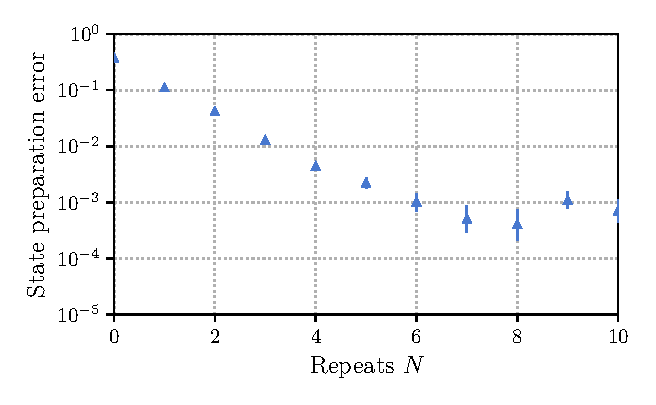
\includegraphics[width=0.75\linewidth]{
            figures/pdf_figure/state_prep.pdf
            }
        \end{center}
        \caption{
            State preparation error as a function of the number of state preparation pulses, $N$. The error is defined as population not in the $\ket{\downarrow}$ state after the preparation sequence has been applied. The error is reduced to below $10^{-3}$ after $N=7$ pulses, which is used in our experiments.
            }
        \label{fig:stateprep}
    \end{figure}

\begin{table}
    \begin{center}
    \begin{tabular}{|c|l|}
        \hline
        Parameter & Value \\
        \hline
        729-nm laser power & 1000~\unit{\uW}\\
        729-nm laser detuning & 0~\unit{\MHz}* \\
        729-nm pulse duration & 5~\unit{\us} \\
        854-nm laser power & 60~\unit{\uW}, $250\times I_{\rm SAT}$\\
        854-nm laser detuning & 0~\unit{\MHz} \\
        854-nm pulse duration & 40~\unit{\us} \\
        866-nm laser power & 15~\unit{\uW}, $\sim 70\times I_{\rm SAT}$\\
        866-nm laser detuning & 0~\unit{\MHz} \\
        866-nm pulse duration & 30~\unit{\us} \\
        \hline
    \end{tabular}
    \end{center}
    \caption{
        * With respect to qubit transition frequency.\\
        Experimental parameters used for state preparation of the ion into the $\ket{\downarrow} = \ket{4S_{1/2},~m_j = -1/2}$ state.
        }
    \label{tab:state_prep_parameters}
\end{table}

    To utilise two levels of the ion as a qubit, the electronic state must first be prepared into the qubit manifold. Here, the ion is prepared into the $\ket{\downarrow}=\ket{4S_{1/2},~m_j=-1/2}$ state. 
    This is done via effective optical pumping by pulsing the quadrupole transition $\ket{4S_{1/2},~m_j = +1/2} \leftrightarrow \ket{3D_{5/2},~m_j = -3/2}$,
    followed by deshelving pulses using the 854-nm, 866-nm
    lasers on resonance.  The 729-nm laser pulse duration and intensity is set to invert the populations, i.e. perform a $\pi$-pulse. Details for laser parameters are summarised in table~\ref{tab:state_prep_parameters}. These three pulses are repeated $N$ times sequentially. Figure~\ref{fig:stateprep} shows the state preparation error with increasing $N$. The error is found by applying a $\pi$-pulse on the state preparation transition directly after the state preparation sequence and looking at the population in the $\ket{\downarrow}$ state. Any reduction from $\ket{\downarrow} = 1$ indicates residual population in the $\ket{4S_{1/2},~m_j = +1/2}$ state, or the $D$ levels. After $N=7$ pulses, which is used in our experiments, there is a state preparation error of $<10^{-3}$. This is further verified by randomised benchmarking in section~\ref{sec:Single Qubit Gates}. The state preparation error is likely limited by accidental excitation of the $\ket{4S_{1/2},~m_j = -1/2}$ state to the $D_{5/2}$ level. This may be due to off-resonant excitation of another transition, or due to spectral purity of the 729-nm laser. \\
    Another protocol for state preparation is optical pumping on the dipole transition (397-nm), which often is much faster. However, in this setup it is impractical as polarisation selectivity of the 397-nm transition is not possible due to 
    the constraint of beam geometry from the in vacuum optics, see section~\ref{sec:Vacuum System},
    and frequency selectivity is not possible due to the low magnitude fixed B-field providing Zeeman shifts less than the natural linewidth of the 397-nm transition, see section~\ref{sec:Magnetic Field}. 


\subsection{Measurement}
\label{sec:Measurement}
% Main points:
    % Readout characterisation with NA 0.6 lens
    % Compare readout histograms of fast 30 us readout to Doppler cold 100 us readout
    \begin{figure}
        \begin{center}
        \noindent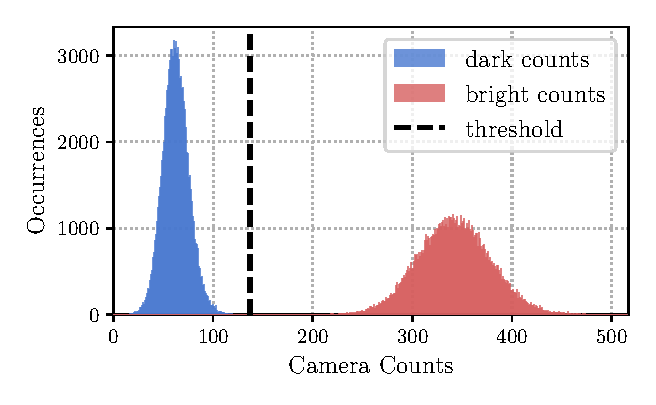
\includegraphics[width=0.75\linewidth]{
            figures/pdf_figure/readout_hist.pdf
            }
        \end{center}
        \caption{
            Readout histogram with 100,000 individual measurements for bright (red) and dark (blue) populations. The camera counts are presented as a histogram and fitted to Poissonian distributions to calibrate a threshold for discerning if the ion is bright or dark with the lowest probability for false measurement. Dark counts are mainly due to 397-nm light scattered from the nearest trap electrodes. With 100~\unit{\us} readout duration, and laser parameters set to Doppler cooling parameters, a threshold count of 137 photons is found, giving an expected statistical error of $6\times 10^{-9}$ given the fitted Gaussians. %Gaussian dark: mean = 62, $\sigma$ = 13. Gaussian bright: mean = 341, $\sigma$ = 36.
            }
        \label{fig:readout_histogram}
    \end{figure}

    \begin{table}
        \begin{center}
        \begin{tabular}{|c|l|}
            \hline
            Parameter & Value \\
            \hline
            397-nm laser power & 3~\unit{\uW}, $1\times I_{\rm SAT}$ \\
            397-nm laser detuning & -17.5~\unit{\MHz}\\
            866-nm laser power & 15~\unit{\uW}, $\sim 70\times I_{\rm SAT}$\\
            866-nm laser detuning & 0~\unit{\MHz} \\
            Doppler cooling duration & 1000~\unit{\us}\\
            Readout duration & 100~\unit{\us} \\
            Camera threshold & 137 counts \\
            \hline
        \end{tabular}
        \end{center}
        \caption{
            Experimental parameters used for Doppler cooling and state-selective fluorescence of the ion. 
            }
        \label{tab:397_parameters}
    \end{table}

    To measure the qubit state, the 397-nm and 866-nm lasers
    are applied, and the scattered 397-nm photons are imaged by the objective onto a camera (see section~\ref{sec:Imaging System}). 397-nm light will only be scattered if the qubit is in $\ket{\downarrow}$.
    Use of a high numerical aperture (NA = 0.6) objective greatly increases the collection efficiency.
    This efficiency allows the 397-nm beam to be red-detuned to Doppler cooling parameters (see section~\ref{sec:Cooling}), while still maintaining low readout duration (100~\unit{\us}) and low readout error. 
    Cooling during readout increases the experiment's repetition rate by reducing the amount of dedicated cooling time required.\\
    The parameters used for readout are
    summarised in table~\ref{tab:397_parameters}, and a typical histogram of
    readout counts for one ion can be seen in
    figure~\ref{fig:readout_histogram}. The readout threshold is calibrated by taking bright counts with the 397-nm and 866-nm lasers on, and dark counts with the 397-nm laser on and the 866-nm laser off. This assumes dark counts are due to 397-nm scattering from the trap electrodes. 
    Fitting Poissonian distributions to the bright and dark measurements, an optimal count threshold of
    137 is found, shown by black dashed line. This threshold gives an expected
    statistical readout error of $\epsilon_\downarrow = \epsilon_\uparrow = 6\times10^{-9}$, where $\epsilon_{\downarrow,\uparrow}$ are the expected error associated with measuring bright or dark. This measurment ignores errors due to the
    finite lifetime of the metastable $3D_{5/2}$ level, which dominate $\epsilon_\uparrow$. The expected error due
    to the finite lifetime, $\tau$, is $\epsilon_{\rm decay} = 1 - e^{-t/\tau}$, where $t$ is the readout duration. For \ca, $\tau \sim 1.1$~s, $\epsilon_\uparrow \approx \epsilon_{\rm decay}  = 
    10^{-4}$. 
    Assuming the metastable lifetime is limited only by spontaneous decay overlooks leakage from the 854-nm deshelving beam, which could significantly shorten $\tau$~\cite{sotirova2024high-fidelity}. \\
    
\subsection{Single Qubit Rotations}
\label{sec:Single Qubit Gates}
% Main points:
    % Here is a characterisation of single qubit gates.
    % Explain RBM method
    % Quote values measured
    % What is likely error source
    % Are we limited by this error?
    % What is state of the art (for optical quadrupole transition)
    % What contribution is the spin coherence time?
% Pre reqs:
    % Spin coherence times
    % Possible transitions
    % Calibrating gate times
    A qubit is fully described by $\ket{\psi} = \alpha\ket{\downarrow} + \beta\ket{\uparrow}$, where $\alpha$ and $\beta$ are complex numbers satisfying $|\alpha|^2 + |\beta|^2 = 1$. The qubit state can be manipulated by applying single qubit rotations, $R_{x,y}(\theta)$, commonly referred to as gates. In the Bloch sphere, $x$- and $y$-rotations are performed by pertubations resonant with the qubit transition, here, using the 729-nm laser. The rotation angle, $\theta$, is given by $\theta=\Omega t/2$, where $\Omega$, is the Rabi frequency, and $t$ is the pulse duration. The rotation axis, is determined by the relative phase of the light field and the qubit. We define the initial relative phase to correspond to a $y$-rotation.

\subsubsection{Gate Time Calibration}
% Main points:
    % The ion is a sensor!
    % Method for Rabi and Ramsey scans
    % Mention changing polarisation to select certain transitions
    % Long Rabi flop
    % Likely reason for flop damping
    % Measuring detuning using Ramsey scan
% Pre reqs:
    % 729 system
    % Available Quadrupole transitions

    \begin{figure}
        \begin{center}
        \noindent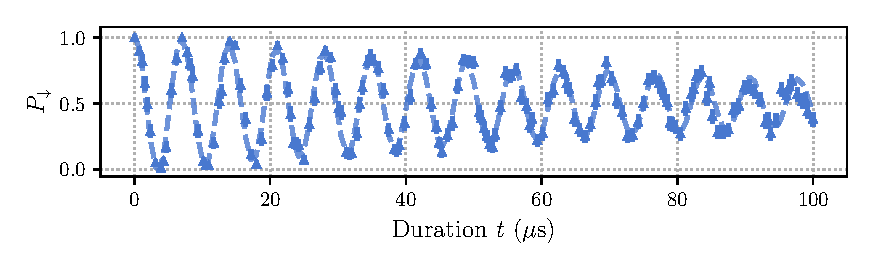
\includegraphics[width=\linewidth]{
            figures/pdf_figure/long_flop.pdf
            }
        \end{center}
        \caption{Long duration, $t$, Rabi flop on the qubit transition to extract Rabi frequency. Estimated probability of being in $\ket{\downarrow}$, $P_\downarrow$, at each time step using 200 individual experimental shots. Fitted dotted line using decaying oscillation model. Extracted Rabi frequency $\Omega/2\pi = 0.2864(2)$~\unit{\MHz}, and decay rate $\lambda = 0.0107(7)$~\unit{\per\us}. 
            }
        \label{fig:Long Flop}
    \end{figure}

    The pulse duration, for a $R(\pi/2)$ ($\pi/2$-pulse), is calibrated by Rabi oscillations. Figure~\ref{fig:Long Flop} shows the population in $\ket{\downarrow}$, $P_\downarrow$, calculated from 200 experimental shots.
    To find the Rabi frequency, $\Omega$, the data is fitted to a decaying oscillation model,
    \begin{equation}
        P_{\downarrow} = \frac{1 + e^{-\lambda t} \cos(\Omega t/2)}{2},
    \end{equation}
    where $\lambda$ is the decay rate due to decoherence
    effects~\cite{wineland1998experimental}. The Rabi frequency is found to be
    $\Omega/2\pi = 0.2864(2)$~\unit{\MHz}, and the decay rate $\lambda =
    0.0107(7)~1/\mu$s.
    From this $R(\pi/2) = 1.7$~\unit{\us} can be estimated.
    These measurements were taken with 1~mW of 729-nm power,
    with beam radius $\sim$15\unit{\um} at the ion.\\
    

\subsubsection{Randomised Benchmarking}

    \begin{figure}
        \begin{center}
        \noindent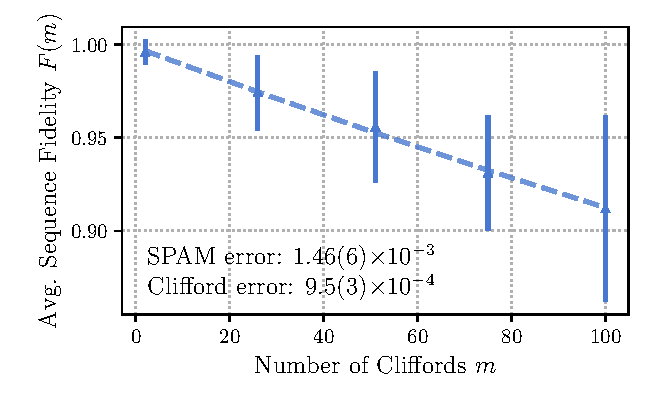
\includegraphics[width=0.75\linewidth]{
            figures/pdf_figure/rbm_fit.pdf
            }
        \end{center}
        \caption{
            Estimating single qubit Clifford fidelities, $\mathcal{F}$, and errors due to state preparation and measurement, using randomised benchmarking. 
            The data points are the average survival population after applying a sequence of $m$ random Clifford gates, and a final inverting Clifford gate. The dashed line is the fit to the decay model given by equation~\ref{eq:RBM_decay}. The error bars are given by the standard deviation of the survival populations.
            }
        \label{fig:rbm}
    \end{figure}

    To evaluate the quality of both our
    state preparation and single qubit rotations, randomised benchmarking
    (RBM)~\cite{knill2008randomized} is employed.  RBM consists of
    applying random combinations of gates from the single-qubit Clifford group to
    estimate an average error per gate. The single-qubit Clifford group is
    the set of unitaries which map the Pauli matrices to one another through
    conjugation. The RBM protocol used here is described in~\cite{hughes2021benchmarking}.
    The sequence of operations is as follows:
    \begin{enumerate}
        \item Prepare the qubit in $\ket{\downarrow}$ via optical pumping, section~\ref{sec:Stateprep}.
        \item Apply a random sequence of $m$ single qubit Clifford gates, where $m$ is the length of the sequence.
        \item Apply a final ``inverting'' Clifford gate, which is chosen such that the full sequence performs the identity operation.
        \item Measure the population in $\ket{\downarrow}$, $P_\downarrow$, via state-selective fluorescence, section~\ref{sec:Measurement}.
        \item Repeat steps 1-4 multiple times to find the average survival population, $\langle P_\downarrow \rangle$.
        \item Repeat steps 1-5 for many different random sequences with a range of sequence lengths, $m$.
        \item Fit the decay of the average survival population, $\mathcal{F}(m) = \langle P_\downarrow(m) \rangle$, to a decay model to find the average error per Clifford gate.
    \end{enumerate}
    The decay model used to find 
    the fidelity versus number of Clifford gates is given by\cite{hughes2021benchmarking},
    \begin{equation}
    \label{eq:RBM_decay}
        \mathcal{F}(m) = \frac{1}{2}\left( 1+(1-2\epsilon_{\rm SPAM})(1-2\epsilon_c)^m\right),
    \end{equation}
    where $\mathcal{F}(m)$ is the fidelity of the sequence of length $m$,
    $\epsilon_{\rm SPAM}$ is the state preparation and measurement error, and
    $\epsilon_c$ is the average error per Clifford gate.  The Clifford gates are decomposed into
    sequences of $\pi/2$- and $\pi$-pulses about either the $x$- or $y$-axes. Up to $m=100$ Clifford gates are probed, and the decay of the fidelity, $\mathcal{F}(m)$, is fit using the above model.
    The error per Clifford is found to be $\epsilon_c = 9.5(3) \times 10^{-4}$,
    while the SPAM error is $\epsilon_{\rm SPAM} = 1.46(6) \times 10^{-3}$. The decay plot for
    this RBM sequence can be seen in figure~\ref{fig:rbm}.
    The independently characterised state preparation (section~\ref{sec:Stateprep}) and measurement (section~\ref{sec:Measurement}) errors of $\sim 10^{-3}$, and $\sim 10^{-4}$ respectively, are consistent with the measured $\epsilon_{\rm SPAM}$.

\subsection{Spin Coherence Times}
\label{sec:Coherence}
% Main points:
    % Quote coherence times comparing:
        % Mumetal box panels
        % Transitions with diff mag sensitivity
        % FNC/ no-FNC
% Pre reqs:
    % MuMetal box
    % Available transitions
    % 729 laser system
    \begin{figure}
        \begin{center}
        \noindent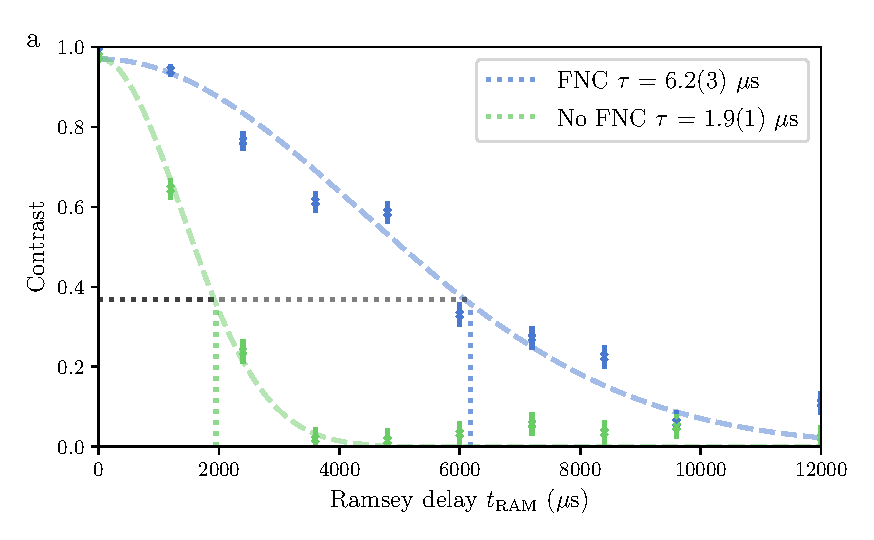
\includegraphics[width=\linewidth]{
            figures/pdf_figure/fnc_coherence.pdf
            }
        \noindent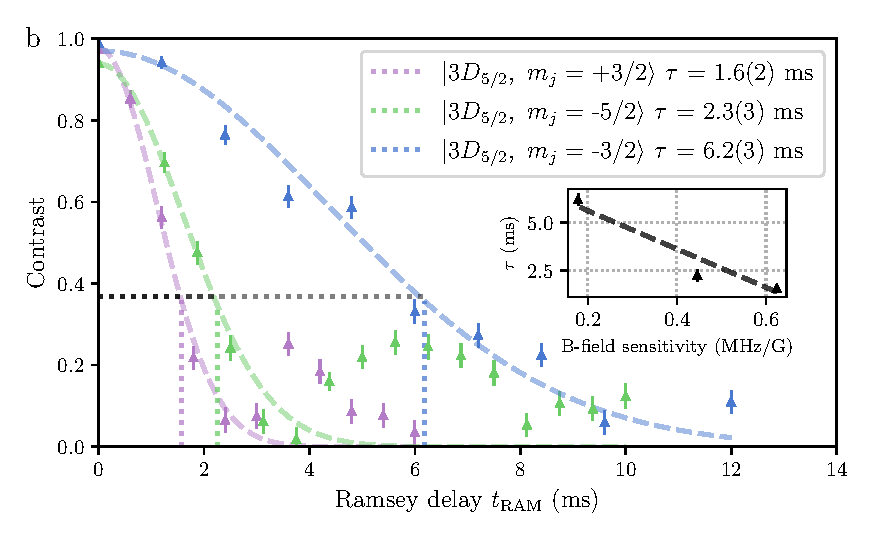
\includegraphics[width=\linewidth]{
            figures/pdf_figure/mag_coherence.pdf
            }
        \end{center}
        \caption{Coherence time measurements.
        \textbf{a)} Coherence time of the $\ket{4S_{1/2},~m_j=-1/2}\leftrightarrow\ket{3D_{5/2},~m_j=-3/2}$ transition with and without fibre noise cancellation (FNC). 
        \textbf{b)} Coherence time of three quadrupole transitions with varying magnetic field sensitivities. The inset plot shows a linear fit between the coherence time and the magnetic field sensitivity of the transition.
            }
        \label{fig:coherence_times}
    \end{figure}
    Decoherence, as can be seen in figure~\ref{fig:Long Flop}, can be caused by laser frequency and power fluctuations, magnetic field noise, and spontaneous emission from the $3D_{5/2}$ level. The coherence time of the qubit is a useful diagnostic for finding unwanted noise sources, and for benchmarking the performance of the qubit as a store of quantum information.\\
    To measure the coherence times, we perform Ramsey sequences with varying delay durations. The Ramsey sequence is as follows:
    \begin{enumerate}
        \item Prepare the qubit in $\ket{\downarrow}$ via optical pumping, section~\ref{sec:Stateprep}.
        \item Apply a $R_y(\pi/2)$ pulse to prepare the qubit in $\ket{+} = \frac{1}{\sqrt{2}}(\ket{\downarrow} + \ket{\uparrow})$ superposition state.
        \item Wait for a time $t_{\rm RAM}$.
        \item Apply a second $R_\phi(\pi/2)$-pulse, with a variable axis of rotation, $\phi$. 
        \item Measure the population in $\ket{\downarrow}$, $P_\downarrow$, via state-selective fluorescence, section~\ref{sec:Measurement}.
        \item Repeat steps 1-5 for different values of $\phi$ and fit the resulting fringe to find the contrast.
        \item Repeat steps 1-6 for different values of $t_{\rm RAM}$ to find the decay in contast with time. The coherence time is defined as the time at which the contrast has decayed to $1/e$ of its initial value.
    \end{enumerate}
    With this tool, the efficacy of the fibre noise cancellation (FNC, see section~\ref{sec:Narrow Line Width 729 Laser}) can be measured. Figure~\ref{fig:coherence_times} $a$ shows the coherence time of the $\ket{4S_{1/2},~m_j=-1/2}\leftrightarrow\ket{3D_{5/2},~m_j=-3/2}$  transition with and without FNC. The coherence time is increased from 1.9(1)~\unit{\ms} to 6.2(3)~\unit{\ms} with FNC, showing that without FNC, the coherence times are limited by laser phase noise. \\
    With FNC enabled, to see if the coherence time is now limited by magnetic field noise, transitions with varying magnetic field sensitivities are compared. Figure~\ref{fig:coherence_times} $b$ shows the coherence time of three quadrupole transitions with varying $D_{5/2}$, $m_j$ numbers: $\ket{4S_{1/2},~m_j=-1/2} \leftrightarrow \ket{3D_{5/2},~m_j=\lbrace -5/2, -3/2, +3/2}$. These transitions have magnetic field sensitivities $-0.446$, $-0.178$, $+0.624$~\unit{\MHz\per\gauss} respectively. The contrast decays for all three qubits are shown in the figure. The inset plot shows a well correlated linear fit between the coherence time and the magnetic field sensitivity, suggesting that the coherence time is limited by magnetic field noise. For both $\ket{4S_{1/2},~m_j=-1/2} \leftrightarrow \ket{3D_{5/2},~m_j=-5/2}$ and $\ket{4S_{1/2},~m_j=-1/2} \leftrightarrow \ket{3D_{5/2},~m_j=+3/2}$, revivals in contrast can be seen which suggest that the dominant noise source is oscillatory and coherent over the Ramsey scan duration.\\
    These measurements were taken without the MuMetal enclosure (section~\ref{sec:Magnetic Field}) fully assembled around the vacuum system, which we expect will greatly reduce external magnetic field noise, and therefore increase the coherence times.


\section{Motion}
\label{sec:Motion}
% Main points:
    % Quote characterisation method and values for various motional measurements.
    % Highlight where we are not yet at the capability we need.
    % State what improvements we plan to add.
% Pre reqs:
    % Motivation for control of motion of ion
    % Trap RF DC
    % Laser systems

    Motion of ions trapped in the same potential can be described by a set of normal modes~\cite{james1998quantum}. These modes are labelled with respect to the ion chain geometry: axial modes oscillate parallel with the chain, and radial modes oscillate perpendicular to the chain. Due to the geometry of the 729-nm beam access with respect to the ion chain (see section~\ref{sec:Vacuum System}), only the radial modes can be addressed in our system. For the \emph{NPL} trap (see section~\ref{sec:The Ion Trap}), the radial modes frequencies are non-degenerate. In our system, for a single ion, the radial mode frequencies are $\omega_{\rm upper}/2\pi = 4.0$~\unit{\MHz}, and $\omega_{\rm lower}/2\pi = 2.5$~\unit{\MHz}, and the axial mode frequency is $\omega_{\rm axial}/2\pi = 1.6$~\unit{\MHz}. All work here is using the upper radial mode. \\
    The motional mode, $i$, leads to sidebands in the 729-nm spectrum at $\omega_0 \pm \omega_{i}$~\cite{ozeri2011tutorial}, where $\omega_0$, the carrier, is the frequency of the 729-nm laser when on resonance with the qubit transition. The $+\omega_i$ sideband is referred to as the blue sideband (BSB), and the $-\omega_i$ is the red sideband (RSB).
    The RSB, BSB, and RF fields near to resonance with the motional modes, are the tools used in this section to manipulatie the motion of the ion.\\
    The motional state preparation, heating rate, frequency stabilities, and coherence times are characterised in this section.

\subsection{Cooling}
\label{sec:Cooling}
% Main points:
    % Introduce why we want to cool
    % Doppler cooling
    % Sideband cooling
% Pre reqs:
    % Motional mode and beam geometry
    % Laser systems 
    % Trapping

    For any interaction that involves the motion of the ion, it is essential to both prepare and measure the motional state with high fidelity. For all motional interactions considered in this thesis, the ion is initially prepared as close as possible to the motional ground state, with a mean phonon number $\bar{n} \approx 0$. This is done by an initial stage of Doppler cooling, followed by pulsed sideband cooling on the 729-nm transition. The final motional state is characterised by measuring the population in Fock states using RSB and effective BSB pulses.\\

\subsubsection{Doppler Cooling}
% Main points:
    % Quote final temperature reached (theory?)
    % Describe cooling parameters
% Pre reqs:
    % Motional mode and beam geometry
    % Laser systems 

    Doppler cooling relies on the fact that light incident on a moving ion 
    appears frequency-shifted in the ion's rest frame. For Doppler cooling
    of \ca, both the 397-nm and 866-nm lasers are applied. The 397-nm laser is red-detuned from the dipole $\ket{4S_{1/2}}\leftrightarrow\ket{4P_{1/2}}$ transition, leading to preferential
    scattering of 397-nm photons that have a net cooling effect~\cite{wineland1979laser}. The excited $4P_{1/2}$ level decays via two channels: emission of a 397-nm photon back to $\ket{4S_{1/2}}$, or an 866-nm photon to $\ket{3D_{3/2}}$, with a branching
    ratio of 14.5~\cite{ramm2013precision}. Since many photon scattering events are required, the cooling cycle must be closed. To prevent population trapping in the metastable $\ket{3D_{3/2}}$ level, the 866-nm laser is applied on resonance during cooling.\\
    Equilibrium
    is reached when the cooling rate balances
    photon recoil heating. Assuming the 397-nm transition is broadened only by its natural linewidth $\gamma$, 
    the minimum Doppler temperature is,
    \begin{equation}
    T_{\rm Doppler} \approx \frac{\hbar\gamma}{2k_B},
    \end{equation}
    where $\hbar$ is the reduced Planck constant, and $k_B$ is Boltzmann's constant~\cite{wineland1979laser}.\\
     For
    $^{40}$Ca$^+$, the natural linewidth of the 397-nm transition is $\frac{\gamma}{2\pi} =
    21$~\unit{\MHz}\cite{morton2003atomic}, giving $T_{\rm Doppler} = 0.5$~\unit{\milli\kelvin}. For a radial mode frequency of $\frac{\omega}{2\pi} = 4$~\unit{\MHz}, the expected mean phonon number is,
    \begin{equation}
        \bar{n} = \frac{1}{e^{\hbar\omega/k_B T}-1},
    \end{equation}
    yielding $\bar{n} = 2.3$ at the Doppler limit.
    The parameters used here for Doppler cooling are summarised in table~\ref{tab:397_parameters}. \\

\subsubsection{Sideband Cooling}
% Main points:
    % Quote final temperature reached
    % Describe SBC pulse sequence
    % We use a closed transition
% Pre reqs:
    % Motional mode spectra
    % Laser systems 
    % Rabi flopping

    \begin{figure}
        \begin{center}
        \noindent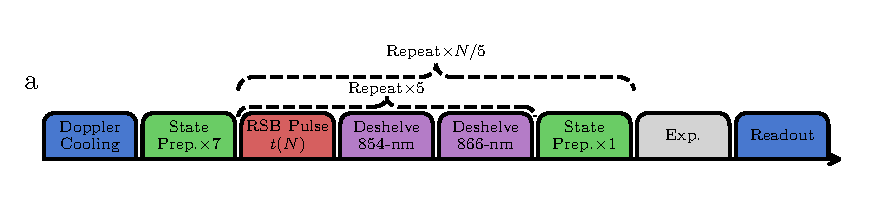
\includegraphics[width=\linewidth]{
            figures/pdf_figure/pulse_sequence.pdf
            }
        \noindent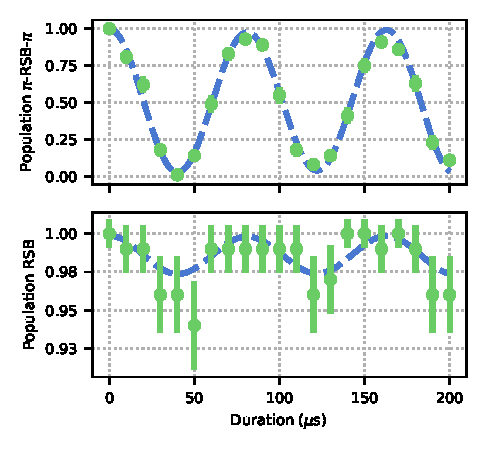
\includegraphics[width=0.75\linewidth]{
            figures/pdf_figure/sideband_thermometry.pdf
            }

        \end{center}
        \caption{
            \textbf{a)} Example pulse sequence for one experimental shot including pulsed sideband cooling. The \emph{Exp.} block represents an arbitrary sequence of operations, for the experiment under study, such as a thermometry sequence.
            The blue blocks represent Doppler cooling and readout (section~\ref{sec:Measurement}), the green blocks represent qubit state preparation (section~\ref{sec:Stateprep}), the red blocks are RSB pulses with varying durations $t(N)$, and the purple blocks are deshelving pulses. After every 5 sideband cooling pulses, there is an interleaved state preparation sequence to ensure there is no population trapped outside of the closed cooling cycle. The RSB length is linearly increased with pulse number $N$, upto the expected RSB $R(\pi)$-pulse duration for $n=1$.  
            \textbf{b, c)} Thermometry scans after Doppler and sideband cooling. The red points are the populations measured via on-resonance RSB pulses, and the blue points are the populations after a sequence of $R(\pi)$-RSB-$R(\pi)$ with varying RSB probe durations. The dashed lines are fits to a thermal Fock state distribution, with truncation at $n = 100$. The extracted mean occupation number is $\bar{n} = 0.03(1)$, and $\eta\Omega/(2\pi) = 11.6(1)$~\unit{\kHz}. 
            }
        \label{fig:SBC}
    \end{figure}
    \begin{table}
        \begin{center}
        \begin{tabular}{|c|l|}
            \hline
            Parameter & Value \\
            \hline
            729-nm laser power & 3.0~\unit{\mW}\\
            729-nm laser detuning & -4.0~\unit{\MHz}*\\
            729-nm pulse duration $N = 1$ & 2.5~\unit{\us}\\
            729-nm pulse duration $N = N_{\rm max}$ & 33~\unit{\us}  \\
            Repumping 866-nm duration & 14~\unit{\us}\\
            Deshelving 854-nm duration & 5~\unit{\us}\\
            Number of cooling cycles $N_{\rm max}$ & 50\\
            \hline
        \end{tabular}
        \end{center}
        \caption{
            *729-nm detuning is relative to the $\ket{4S_{1/2},~m_j=-1/2} \leftrightarrow \ket{3D_{5/2},~m_j=-5/2}$ transition frequency.\\
            Experimental parameters used for sideband cooling. Other parameters for the repump and deshelve pulses are the same as for state preparation, see table~\ref{tab:state_prep_parameters}. The 729-nm laser is detuned to the RSB resonance for the upper radial mode, $\omega_{\rm upper}/2\pi = 4.0$~\unit{\MHz}, and the pulse duration for $N=N_{\rm max}$ is chosen to be the expected RSB $R(\pi)$-pulse duration for $n=1$. 
            }
        \label{tab:sbc_parameters}
    \end{table}

    To further cool the ions toward their motional ground state, resolved
    sideband cooling is used. As mentioned above, the motion of the ion
    modulates the absorption spectrum of the ion, leading to red and blue sidebands (RSB and BSB). For the $\ket{4S_{1/2}} \leftrightarrow
    \ket{3D_{5/2}}$ transition, at appropriate motional mode
    frequencies, interaction strengths, and using a narrow linewidth laser (section~\ref{sec:Narrow Line Width 729 Laser}), these sidebands can be resolved spectroscopically. The pulsed
    sideband technique employed consists of RSB pulses on the 729-nm transition, followed by
    deshelving, and repumping pulses on the 854-nm and 866-nm transitions
    respectively. 
    For efficient cooling, initial short 729-nm pulses are applied to preferentially excite the thermal population with high phonon number, as the pulse duration for RSB $R(\pi)$ is proportional to $\sqrt{n}$, where $n$ is the phonon number.  The RSB pulse length is linearly increased to the expected RSB $R(\pi)$-pulse duration for $n=1$.\\
    An example pulse sequence for a single experimental shot using sideband cooling, can be seen in
    figure~\ref{fig:SBC} $a$. Experimental parameters used are summarised in table~\ref{tab:sbc_parameters}.\\
    To verify the efficacy of our sideband cooling, thermometry
    experiments are performed by probing Fock state populations. This is done using on resonance RSB pulses and effective BSB pulses composed of a $\pi$-RSB-$\pi$ pulse
    sequences. The time dynamics of population flopping is measured as RSB
    pulse length, $t$, is varied. In the case of Fock state $\ket{0}$, there should be full contrast 
    ``BSB'' oscillations, and no visible oscillations when probed with RSB pulses. A thermal
    Fock state distribution~\cite{meekhof1996generation} (with truncation at Fock state = 100) is fitted to these
    signals to extract the mean occupation number, and $\eta\Omega$, the carrier
    Rabi frequency multiplied by the Lamb-Dicke parameter. A typical thermometry
    scan after Doppler and sideband cooling can be seen in
    figure~\ref{fig:SBC} $b, c$, where $b$ shows the population after effective ``BSB'' pulses, and $c$ shows the population after RSB$(t)$ pulses with duration $t$. These oscillations are fit to thermal Fock state distributions, shown by the dashed lines. The mean occupation
    number after sideband cooling is found to be $\bar{n} = 0.03(1)$, and $\eta\Omega =
    11.6(1)$~\unit{\kHz}.\\

    %Optimisation of the cooling parameters can be roughly performed by fitting
    %temperature while scanning RSB $\pi$-pulse durations, total number of pulses,
    %repumping and deshelving times. One can optimise for minimum temperature,
    %however it is also important to optimise for total cooling duration. For
    %single ion, single mode experiments, this duration is often not a limiting factor for experimental run-times,
    %however for multi-ion crystals, any interaction involving the motion may
    %require the sequential sideband cooling of multiple motional modes. This can
    %not be easily parallalised due to the requirement that the RSB $\pi$-pulse is
    %performed near resonance to one of the motional sidebands. This sequential
    %cooling strategy can be either limiting when heating and cooling rates are
    %comparable, or lead to prohibitive data acquisition times.\\
    %To mitigate this issue, other sub-Doppler cooling techniques with larger
    %accepted mode frequency bandwidths may be employed. Examples are dark-resonance
    %cooling~\cite{reis1996cooling,allcock2016dark-resonance}, electromagnetically induced transparency (EIT) cooling~\cite{roos2000experimental}, and
    %Sisyphus cooling~\cite{cirac1992laser}. These techniques are not yet implemented in our system,
    %but will be likely additions once we move to larger ion crystals.\\

\subsection{Heating Rates}
\label{sec:Heating}
% Main points:
    % Quote motional heating rates for mode we use (have access to).
    % Describe heating model?
% Pre reqs:
    % Thermometry
    % Motional modes
    % Trap

    \begin{figure}
        \begin{center}
        \noindent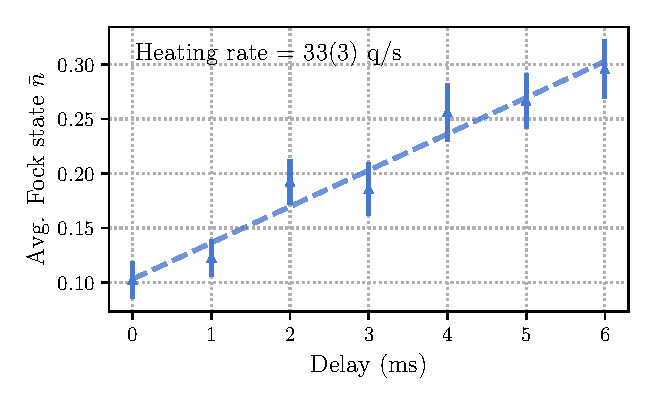
\includegraphics[width=0.75\linewidth]{
            figures/pdf_figure/heating_rate.pdf
            }
        \end{center}
        \caption{
            Heating rates of upper radial mode, measured by varying the delay between cooling and thermometry pulses. The dashed line is a linear fit to the data, with slope $33(3)$~quanta/s. The error bars are given by the standard deviation of the fitted $\bar{n}$.
            }
        \label{fig:heating rates}
    \end{figure}

    After cooling the motion, the ion will return to a temperature in equilibrium with the environment. However, this process can be slowed by adequate isolation of the ion. In UHV ion trap systems (see section~\ref{sec:Vacuum System}), motional heating is predominantly caused by electric field noise from the ion trap~\cite{wineland1998experimental}. Noise due to thermal charge fluctuations at the trap surface can be 
    mitigated by increasing ion-electrode distances. The \emph{NPL} trap (section~\ref{sec:The Ion Trap}), used here, has an ion-electrode 
    distance of 250~\unit{\um}, larger than most surface traps, but less than that of a
    macroscopic blade or rod style trap~\cite{milne2021construction}. Heating rates were probed by a series of thermometry experiments, explained above, with varying delay
    times, $t_{\rm delay}$, between cooling and thermometry pulses. A typical plot can be seen in
    figure~\ref{fig:heating rates}. The heating rate of the system
    was found by a linear fit, shown by the dashed line, to be $33(3)$~quanta per second on the upper radial 4~\unit{\MHz} mode on
    one ion. As will be discussed in section~\ref{sec:Motional Coherence}, the heating rate sets a limit for the motional coherence time.\\

    %It is expected that the heating rate will be larger for lower frequency
    %motional modes if electric field noise is assumed to be uniform over its spectrum~\cite{}. 
    %We also verify
    %this by looking at heating rate on the radial mode while varying the axial
    %mode frequency. This is a useful diagnostic to check for unexpected heating
    %at certain frequencies, perhaps due to RF noise in the lab. We find....\\

\subsection{Motional Mode Stability}
\label{sec:Motional Mode Stability}
% Main points:
    % Quote motional mode drift 
    % Explain why it is currently drifty
    % Outline how this will be improved with the squareatron
% Pre reqs:
    % Trap

    \begin{figure}
        \begin{center}
        \noindent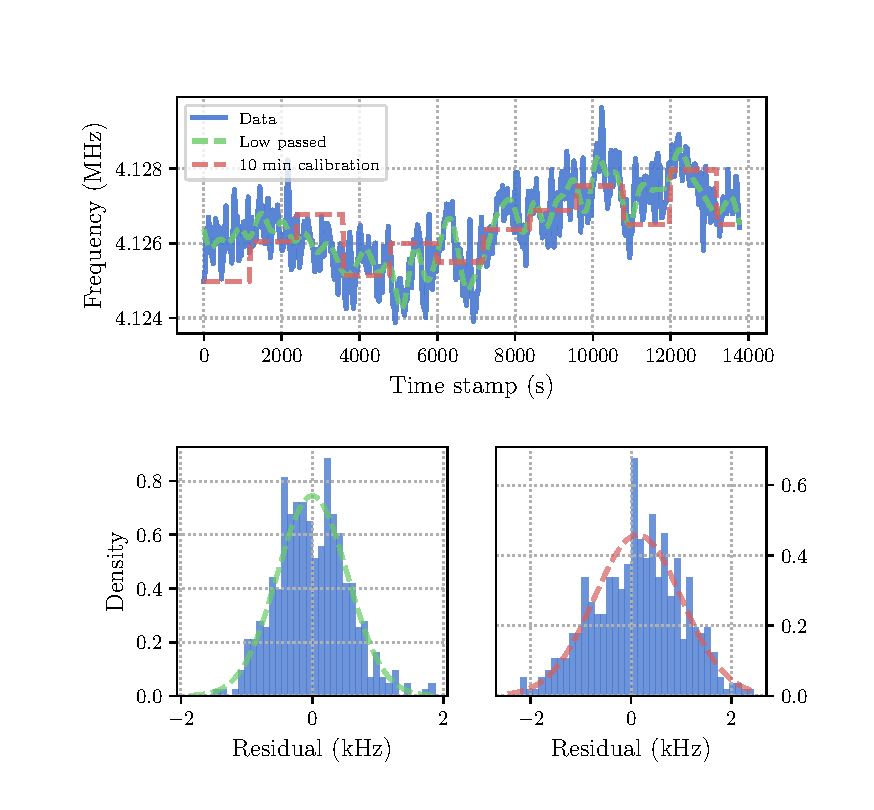
\includegraphics[width=\linewidth]{
            figures/pdf_figure/mode_drift.pdf
            }
        \end{center}
        \caption{
            \textbf{a)} Motional mode frequency drift over time. The radial motional mode frequency is measured by exciting motion using an RF field in resonance with the motional frequency, and looking at increased fluorescence. The resulting frequency trace is shown in blue. The green line shows a low pass filter of the data, with cut-off frequency of 1.67~\unit{\mHz}, corresponding to an assumed 10 minutes slow thermal drift. The motional mode frequency is typically calibrated every 10 minutes, which is indicated by the red line. 
            \textbf{b)} Residuals from the measured data and expected calibrated mode frequencies. The standard deviation of these residuals suggests the typical misset detuning of the mode frequency in current experiments with automated mode frequency calibrations every 10 minutes.
            \textbf{c)} Residuals from the measured data and the low passed trace. The standard deviation of these residuals are due to noise with period less than 10 minutes. 
            }
        \label{fig:mode drift}
    \end{figure}

    Due to thermal drifts and microphonics introducing amplitude and frequency noise on the RF chain, drifts of the radial motional mode frequencies are seen over time. As will be discussed in the following section~\ref{sec:Motional Coherence}, this can lead to dephasing of the motional state. Here, the current motional mode stability is characterised to estimate its contribution to dephasing, and to set a benchmark for future stability improvements. \\
    The motional mode frequency is measured via an RF ``tickle'' experiment. This consists of short ($\sim 5$~\unit{\us}) RF field pulses applied to one of the trap DC electrodes which has a non-zero electric field projection to the mode we wish to probe. The frequency of the RF field is scanned around the expected motional mode frequency, and when resonant, drives the motion of the ion. This resonance is measured by observing an increase in fluorescence counts using a 397-nm laser red-detuned by 100~\unit{\MHz}. To measure mode frequency drift, this sequence is repeated every 10 seconds over multiple hours. A typical plot can be seen in figure~\ref{fig:mode drift} $a$. Over this two hour period, the frequency had an absolute drift of 1.5~\unit{\kHz}. Typically, we calibrate the mode frequency every 10 minutes, which is indicated with the red dashed line. Residuals between this calibrated line and the data, shown in $b$, have a standard deviation of $\sigma/(2\pi) = 203(8)$~\unit{\Hz}, giving the expected uncertainty of the mode frequency detuning given our current periodic calibration routine. A slow drift with frequency cut-off of 1.67~\unit{\mHz} is also fitted to the data, shown in green. The residuals from this fit, shown in $c$, have a standard deviation of $\sigma/(2\pi) = 94(4)$~\unit{\Hz}. This suggests that the motional mode frequency is relatively stable over time scales shorter than 10 minutes, but has a slow drift on longer time scales, which is likely due to thermal fluctuations. \\
    
    % Tracking noise source
    % Show resonator scan
    % Explain we sit either on peak or edge
    % show mode drift of +- edge of resonator.
    % This suggests amplitude drift
    % XXX However, we can distinguish between amplitude or resonator frequency drifts by changing the trap RF frequency. Figure~\ref{fig: mode drift} shows the motional mode frequency versus the trap RF frequency. The quadratic responce seen is due to the bandwidth of the resonator. By probing two points If the central frequency of the resonator drifts over time
    

\subsection{Motional Coherence Times}
\label{sec:Motional Coherence}
% Main points:
    % Quote measured result for motional coherence time
    % Give estimate for what times we need for future experiments
    % Give estimate contributions from motional heating and from mode instability
    % What fix will we do for improving this - squareatron from prev section, resonator.
% Pre reqs:
    % Trap RF
    % Trap Resonator
    % Motional mode stability
    % SBC
\begin{figure}
    \begin{center}
    \noindent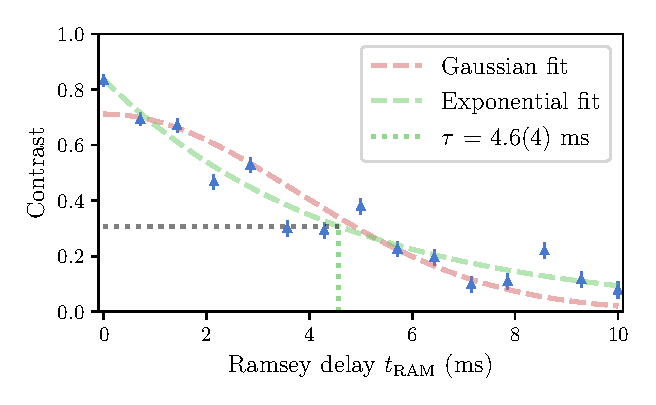
\includegraphics[width=0.75\linewidth]{
        figures/pdf_figure/motional_coherence.pdf
        }
    \end{center}
    \caption{
        Motional coherence time measured by Ramsey sequence on the motional state. The blue points are the population in $\ket{\downarrow}$ after a Ramsey sequence with varying delay time, $t_{\rm RAM}$. The dashed line is an exponential decay fit, with a coherence time $\tau = 4.6(4)$~\unit{\ms}.
        }
    \label{fig:motional_coherence}
\end{figure}

    We will utilise the motional modes of the ion to store quantum information.
    As with the section on spin coherence times~\ref{sec:Coherence}, the
    fidelity of operations, and success probability of algorithms will be
    limited by the coherence time of the motional state.  To measure motional
    coherence, a Ramsey sequence is performed between states $\ket{\downarrow, 0}$
    and $\ket{\downarrow, 1}$, where the first element is the qubit
    state, and the second element is the motional Fock state. To prepare these
    states the following pulse sequence is applied:
    \begin{enumerate}
    \item State prepare system to $\ket{\downarrow, 0}$ via optical pumping and sideband cooling.
    \item Apply $R_y(\pi/2)$-pulse on carrier transition to prepare the qubit in $(\ket{\downarrow, 0} + \ket{\uparrow, 0})/\sqrt{2}$.
    \item Apply $R(\pi)$-pulse on the RSB to prepare the motional state in $(\ket{\downarrow, 0} + \ket{\downarrow, 1})/\sqrt{2}$.
    \item Delay for some time $t_{\rm RAM}$.
    \item Apply $R(\pi)$-pulse on the RSB to map accumulated phase onto the qubit state.
    \item Apply $R_\phi(\pi/2)$-pulse on the carrier, with variable axis of rotation, $\phi$.
    \item Measure the population in $\ket{\downarrow}$ via state-selective fluorescence, section~\ref{sec:Measurement}.
    \item Repeat steps 1-7 for different values of $\phi$ to find the contrast of the Ramsey fringe.
    \item Repeat steps 1-8 for different values of $t_{\rm RAM}$ to find the decay in contrast with time. The coherence time is defined as the time at which the contrast has decayed to $1/e$ of its initial value.
    \end{enumerate}
    There are two main mechanisms for motional decoherence\cite{turchette2000decoherence}: motional heating, as
    characterised in section~\ref{sec:Heating}, and motional dephasing due to
    mode frequency instability, as discussed in section~\ref{sec:Motional Mode Stability}. \\
    A heating rate dominated coherence time is given by, $\tau_{\rm HEAT} =
    (\sqrt{e}-1)/\dot{\bar{n}}$~\cite{turchette2000decoherence}, where $\dot{\bar{n}}$ is the heating
    rate. A dephasing dominated coherence time, if noise is correlated on timescales long compared to the Ramsey delay~\cite{omalley2015qubit}, is characterised by a Gaussian decay profile with a coherence time
    of $\tau_{DEPH} = \sqrt{2}/\sigma_{\omega}$.\\
    Evaluating both of these models with $\dot{\bar{n}}=33(3)$~q/s, and
    $\sigma_{\omega}/(2\pi) = 94(4)$~\unit{\Hz}, the expected motional coherence times of $\tau_{\rm
    HEAT} \approx 20$~ms and $\tau_{\rm DEPH} \approx 2.3$~ms respectively, are found. From these auxiliary characterisations of the motional modes, it is expected that the coherence time will be limited by motional dephasing. \\
    Figure~\ref{fig:motional_coherence} shows the decaying coherence when probed by the above sequence. It can be seen that the contrast has a good fit assuming an exponential decay (green dashed line),
    defined by $C(t_{\rm RAM}) = C(0) e^{-t_{\rm RAM}/\tau},$ where $C(t_{\rm RAM})$ is the contrast at time $t_{\rm RAM}$, and $\tau$ is the coherence time. The fit yields a motional coherence time of $\tau = 4.6(4)$~\unit{\ms}, defined as the time at which the contrast decays to $1/e$ of its intitial value. 
    An exponential decay suggests that the noise source causing the dephasing is correlated only for durations much shorter than the Ramsey delay times~\cite{omalley2015qubit}.
    The Gaussian decay, (red dashed line), which was appropriate for the previous spin coherence time measurements in section~\ref{sec:Coherence}, is a poor fit here. \\
    
    

    %Work must be done to estimate the fast motional
    %noise, however, first there may be simple improvements that can be made to
    %the RF chain to improve both short and long term motional mode stability.
    %These improvements are described in section~\ref{sec:Trap RF Chain}.\\


\section{Spin-Motion}
    For full control of the spin-motion hybrid system, we require interactions
    that couple the two. Perhaps the simplest of this class of interactions
    are the red- and blue-sidebands (RSB and BSB respectively). The  RSB
    interaction was used previously in the thermometry and sideband cooling
    sections~\ref{sec:Cooling}. The RSB (BSB) consists of a single frequency
    laser tuned at the carrier frequency minus (plus) the motional mode frequency,
    $\omega_m$. The interaction is well described by the (Anti-) Jaynes-Cummings
    Hamiltonian, and effectively couples spin flips with the addition or
    subtraction of a motional quanta depending on the initial spin state. Here,
    another such interaction coupling spin and motion, known as the
    spin-dependent force, SDF, is introduced. 
    While the RSB and BSB interactions couple the spin and motion in the motional Fock basis, the SDF couples them through spin-dependent displacements, thus in a coherent state basis. The direction of the displacement is determined by the spin state and an effective detuning parameter.

\subsection{Spin-Dependent Forces}
\label{sec:Spin-Dependent Forces}
% Main points:
    % This is a primitive for motional control
    % This (we will see), is functionally a primitive for two qubit spin entanglement
    % Show equation as quite key to future work
% Pre reqs:
    % Motional mode spectra
    % 729 system
    % AOM control of 729
    The optical Mølmer-Sørensen (MS) scheme~\cite{sorensen2000entanglement} is used to generate the
    SDF via a bichromatic laser field. Bichromatic refers to the simultaneous
    application of two tones symmetrically detuned around the qubit carrier
    frequency, with absolute detuning approximately equal to the motional mode
    frequency, $\delta \approx \omega_{m}$. The resulting interaction, when
    ignoring off-resonant and higher order couplings, is given by,
    \begin{equation}
        \hat{H}_{MS} = i\hbar \eta\Omega\hat{\sigma}_\phi\cos(\delta t) \left( \hat{a} e^{-i\omega_{m} t} + \hat{a}^\dagger e^{i\omega_{m} t} \right),
    \end{equation}
    where $\eta$ is the Lamb-Dicke parameter, $\Omega$ is the carrier Rabi
    frequency, $\hat{a}(\hat{a}^\dagger)$ is the lowering (raising) operator, and
    $\hat{\sigma}_\phi$ is the Pauli operator with $\hat{\sigma}_\phi = \cos(\phi)\hat{\sigma}_x + \sin(\phi)\hat{\sigma}_y$.
    Applying the rotating wave approximation, and defining $\delta_g = \delta -
    \omega_{m}$, the interaction Hamiltonian can be approximated
    to,
    \begin{equation}
        \label{eqn:MS}
        \hat{H}_{MS} \approx \frac{i\hbar \eta\Omega}{2}~\hat{\sigma}_\phi \left( \hat{a} e^{-i\delta_g t} + \hat{a}^\dagger e^{i\delta_g t} \right).
    \end{equation}
    The trajectory of this displacement can be controlled by varying $\delta_g$: on
    resonance, $\delta_g = 0$, corresponds to linear trajectories, whilst off resonance,
    $\delta_g \neq 0$, corresponds to cyclic trajectories where after some duration $t =
    2\pi/\delta_g$, the motion returns to the initial state (with perhaps some phase shift~\cite{haljan2005spin-dependent}). 
    The dynamics of the SDF may be measured by projective spin measurements, the population in $\ket{\downarrow}$, $P_\downarrow$, after applying the SDF for duration $t$ is described by~\cite{burd2020squeezing},
    \begin{equation}
        \label{eqn:sdf_pop}
        P_{\downarrow,\mathrm{th}} = \frac{1}{2} \left[ 1 + e^{-4\left( \bar{n} + \frac{1}{2} \right) |\alpha(t, \delta_g)|^2} \right],
    \end{equation}
    where $\bar{n}$ is the initial thermal phonon occupation, and $|\alpha(t, \delta_g)| = \Omega_{\rm SDF} \sin(\delta_g t/2)/\delta_g$, is the absoltue displacement of the initial state.
    This control is utilised in both two-qubit entangling gate experiments, as well as
    in the creation of squeezed states.\\

\subsubsection{Calibrating the SDF}
% Main points:
    % Here describe what error sources "look like"
    % Describe detuning and duration scans
    % Describe how we can detect these errors via the above strategy. Refer to OB thesis.
    % Fit an SDF with the errors?
% Pre reqs
    % Motional mode spectra
    % 729 system
    % AOM control of 729

    \begin{figure}
        \begin{center}
        \noindent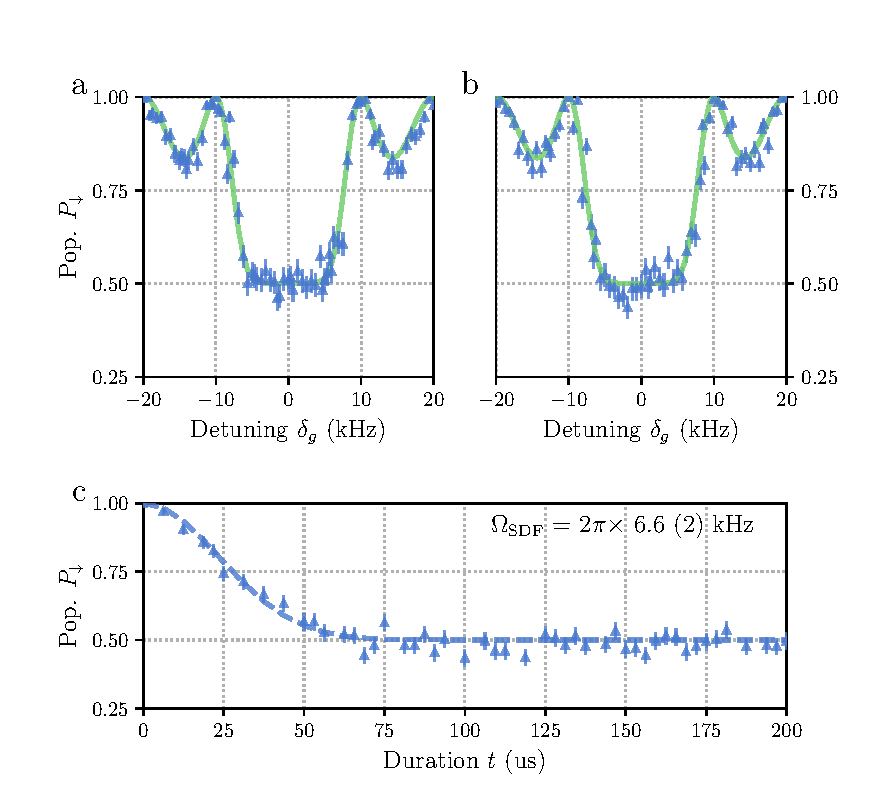
\includegraphics[width=\linewidth]{
            figures/pdf_figure/sdf.pdf
            }
        \end{center}
        \caption{
            Detuning and duration scans of the spin-dependent force applied to an initial thermal state with $\bar{n} = 0.03(1)$. 
            \textbf{a)} Detuning scan, where the detuning, $\delta_g$, is varied, and the duration is fixed at $t=100$~\unit{\us}. The green line is a fit to the expected behaviour given by equation~\ref{eqn:sdf_pop}. 
            \textbf{b)} Detuning scan with a misset qubit frequency of $0.5$~\unit{\kHz}. The green line is the same fit as in $a$ to guide the eye. 
            \textbf{c)} Duration scan, where the duration, $t$, is varied, and the detuning is fixed at $\delta_g = 0$. The dashed line is a fit to the expected behaviour given by equation~\ref{eqn:sdf_pop} with only $\Omega_{\rm SDF}$ as a free parameter.
            }
        \label{fig:SDF}
    \end{figure}

    Geometric phase gates, such as the MS interaction, are widely employed in ion trap experiments due to their robustness against variations in initial motional state. However, the SDF is sensitive to various frequency and power miscalibrations and drifts of these between calibrations.  Here, we describe the workflow for calibrating and optimising the SDF behaviour.\\
    In practice, the SDF interaction involves relatively few degrees of freedom: the central qubit frequency, the motional mode frequency, the power in each tone, and the durations of the pulses must all be calibrated. The complexity comes from the fact that the ion is a multi-level system, posseses multiple motional modes, and that each experimental parameter can only be controlled with finite precision.\\
    The effect of nearby motional modes is negated by either selecting the
    interaction mode to be well seperated from the others either in frequency, by beam geometry, by
    operating the SDF near to resonance of the desired mode, or by using amplitude shaping of the pulse.
    Smoothing a square pulse through amplitude shaping narrows the pulse frequency bandwidth, and thus reduces unwanted off-resonant
    excitation of other modes.  \\
    The power balance of the SDF tones is complicated due to our use of AOMs.
    AOMs generate frequency shifts in the laser beam at the expense of small
    frequency-dependent angular shifts. After the AOM, the beam is coupled into a
    single mode fibre (see figure~\ref{fig:729}), and so the AOMs effectively introduce a
    frequency-dependent loss. To calibrate the power balance, a pick
    off of the bichromatic beam after the ion is monitored on a high bandwidth photodiode.
    The beatnote contrast is measured for the two tones and the power
    balance is optimised by maximising this contrast.\\
    The far off-resonant levels of our ion lead to light-shifts of our qubit
    frequency. To account for the light-shift the central qubit frequency must be calibrated at the
    optical power used for the interaction. This is done with the SDF interaction
    itself. When the qubit frequency is set incorrectly, the two tones will no
    longer have the same absolute detuning from their respective RSB or BSB.
    This manifests as a ``skewness'' of the SDF detuning trace. By varying the qubit frequency and
    inspecting these detuning scans, the desired SDF behaviour can be found. \\
    To verify the behaviour of the calibrated SDF, the experimental data is compared with theory. Both
    ``detuning'' and ``duration'' scans are used. The ``detuning'' scan is performed by
    varying the detuning, $\delta_g$, of the interaction, whilst keeping the
    SDF duration, $t$, constant, and vice-versa for the ``duration'' scan. \\
    Figure~\ref{fig:SDF} $c$ shows the measured duration scan described by equation~\ref{eqn:sdf_pop}, with $\delta_g = 0$ and the the motional state assumed to be thermal with average Fock state $\bar{n}
    = 0.03(1)$ which was found previously from thermometry measurements.
    Here, the displacement, $|\alpha(t)| = \Omega_{\rm SDF} t/2$, where $\Omega_{\rm SDF}$ is the
    SDF amplitude. The dashed line fit is given by floating $\Omega_{\rm SDF}$ only, and finds $\Omega_{\rm SDF}/(2\pi) = 6.6(2)$~\unit{kHz}.
    These measurements were performed with total 729-nm power of 2~mW and $\delta_{\rm LS}/(2\pi) = 3.5$~\unit{\kHz}, the light shift due to the 729-nm laser relative to the unperturbed qubit frequency. \\
    The detuning scan, shown in figure~\ref{fig:SDF} $a$, has the same experimental parameters, but with fixed duration $t=100$~\unit{us}. The fit in green is taking the 
    displacement to be $|\alpha(t)| = \Omega_{\rm SDF} \sin(\delta_g t/2)/\delta_g$, given the value for $\Omega_{\rm SDF}$ measured from the duration scan. Here,
    a qualitatively good agreement between the measured data and the
    expected behaviour is seen, with the main features being the ``closure''
    at $\delta_g = 2\pi/t$ where the motional state returns to the initial state,
    and the central flat region around $P_{\downarrow, \mathrm{th}} =0.5$ where
    the two motional wave packets are non-overlapping.\\
    Figure $b$ shows an example detuning scan when the qubit frequency is misset by $0.5$~\unit{\kHz}. The central region now displays a clear assymmetry around $\delta_g = 0$. The green line here is the fit from $a$ to guide the eye.


\subsection{Two-Qubit Entangling Gates}
\label{sec:Two-Qubit Entangling Gates}
% Main points:
    % Intro/brief outline of goal of two-qubit gate. Truth table? Preparing in Bell state. This is tool kit for spin control of our system.
    % Discuss likely limitations being nearby hot motional modes, no pulse ramping
    % Current error vs what we expect we need for future experiments.
    % Here empasise that the SDF we discuss previously can be used to generate entanglement.
    % Showing phase coherence between operations is nice here.
% Prereqs:
    % SDFs
    % Single qubit gates
    % What available transitions we have
    % Motional mode spectra

    \begin{figure}
        \begin{center}
        \noindent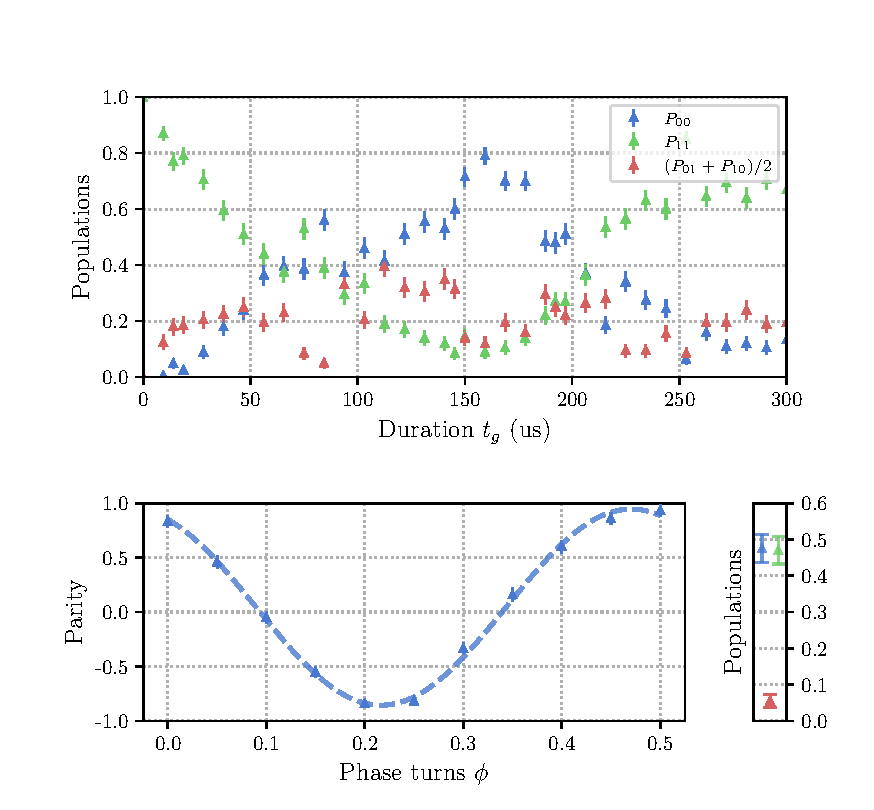
\includegraphics[width=\linewidth]{
            figures/pdf_figure/ms_gate.pdf
            }
        \end{center}
        \caption{
            Experimental data for $\mathcal{F}=92(2)$\% Mølmer-Sørensen (MS) two-qubit entangling gate.
            \textbf{a)} Populations versus duration scan of the MS interaction.
            Each point corresponds to the average of 200 shots, and the error
            bars are given by the standard deviation of these averages. The blue
            points are the populations of both ions being in the $\ket{0}$
            state, $P_{00}$, the green points are the populations of both ions
            being in the $\ket{1}$ state, $P_{11}$, and the red points are the
            ions being the the opposite states, $(P_{01}+P_{10})/2$. The desired
            entangling gate corresponds here to $t_g =  75$\unit{\us}. 
            \textbf{b)} Parity oscillations after the MS interaction. The parity
            is defined as $P_{00} + P_{11} - P_{01} - P_{10}$. The fitted
            contrast here is $0.90(2)$.
            \textbf{c)} Populations at the desired entangling gate duration, $t_g =
            75$~\unit{us}.  
            }
        \label{fig:ms_gate}
    \end{figure}

    We perform two-qubit entangling gates using the Mølmer-Sørensen (MS)
    interaction~\cite{sorensen2000entanglement}. This interaction is the same described SDF from the
    previous section, but applied globally to two ions. The MS interaction
    relies on the spin dependent geometric phase accumulated during the motional
    displacement~\cite{ozeri2011tutorial}. To create a two-qubit entangled state, a differential
    geometric phase of $\pi/2$ must be accumulated between the two-qubit basis
    states~\cite{ozeri2011tutorial}. To ensure there is no residual motional entanglement, the final
    motional state must return to the initial state. In practise, using an SDF
    detuned by $\delta_g$, this is achieved by applying the MS interaction for a
    duration $t_g = 2n\pi/\delta_g$, where $n$ is the number of ``loops''. The MS gate is a universal two-qubit gate, and
    along with only single qubit gates, constitutes a universal gate set for
    discrete quantum algorithms.\\  
    Here we quote the current fidelity of experimentally demonstrated two-qubit gates on
    our system. The fidelity serves to quantify the similarity of
    two density matrices. 
    %---------------
    %For the use case of quantum information processing, what we
    %care about is that the experimental unitary applied in the gate sequence closely resembles the unitary we desire theoretically. In general this
    %means that the fidelity of the applied unitary should be measured in an input
    %state agnostic way. Unfortunately, this is often not practical as the input
    %state space can be unwieldly, and the act of preparing the input state can
    %also be error prone. As a compromise, the unitary is tested with either
    %one, or a set of input states, and the fidelity of the output state
    %is measured with respect to the known target state. 
    %---------------
    %Gate performance, quantified by the fidelity, can be measured by tomography~\cite{}.
    %While full quantum process tomography provides an input-independent measure of fidelity, it is often impractical due to the size of the state space and preparation errors. Instead, the unitary is typically tested on one or a few input states, with fidelity evaluated against the expected output.
    %---------------
    %If the error mechansisms of the 
    %unitary are well understood, arguments can be made that this measured
    %fidelity for a set of input state is representative (or not representative)
    %of the average fidelity over the input state space~\cite{}.\\
    %---------------
    Here for a two-qubit entangling gate, we target the creation of the Bell
    state $\ket{\Phi^+_{\phi_0}} = 1/\sqrt{2} \left( \ket{00} +
    e^{i\phi_0}\ket{11} \right)$, from an initial state of $\ket{00}$, where $phi_0$, is some fixed phase.
    The fidelity between our mixed state $\rho$, and the pure Bell state may be
    given by,
    \begin{equation}
        \mathcal{F} = \bra{\Phi^+_{\phi_0}} \rho \ket{\Phi^+_{\phi_0}} = \frac{1}{2} \left( \rho_{00,00} + \rho_{11,11} \right) + \frac{1}{2}\left( e^{i\phi_0}\rho_{11,00}+e^{-i\phi_0}\rho_{00,11}\right),
        \label{eq:Fidelity}
    \end{equation}
    where $\rho_{ij,kl} = \braket{ij|\rho|kl}$. To extract the fidelity experimentally, a partial state tomography 
    protocol is used~\cite{sackett2000experimental}, where the first bracketted term of
    equation~\ref{eq:Fidelity} is measured by performing projective measurements
    of the two ions after the gate sequence to extract populations, and the second bracketted term,
    known as the coherence terms, are measured by applying a global analysis
    $R_\phi(\pi/2)$ pulse to the two ions and applying parity measurements. 
    Parity measurements are defined as $P = P_{00} + P_{11} - P_{01} - P_{10}$, where $P_{ij}$ is the population of the two ions in state $\ket{i}\ket{j}$ after the gate sequence and variable $\pi/2$-pulse. 
    Creating a Bell state is essential for two-qubit entanglement, but its basis can vary as long as it is consistent across experiments. This allows the Bell state phase, $\phi_0$, to float, which in practice means using only the amplitude of the fitted parity oscillations to compute fidelity, ignoring any phase offset.\\
    The best two-qubit entangling gate fidelity currently achieved on our system is $\mathcal{F}=92(2)\%$. As shown in figure~\ref{fig:ms_gate}, the magnitude of the parity scan was measured to be 0.90(2), while the populations $\left( \rho_{00,00} + \rho_{11,11} \right) = 0.95(2)$. Each population point in these figures are found by taking the average of 200 shots of the gate sequence.\\
    These results serve as both a proof of principle for full spin control on
    our system, but also as a benchmark to which we can compare future system
    improvements.  For future work, we will require the use of this entangling
    gate either as Bell state preparation for input to analogue simulation
    experiments~\cite{bazavan2023synthetic}, or as a primitive gate for the spin component of hybrid
    algorithms~\cite{varona2024towards,brenner2024factoring}.  In both these cases, especially any use that requires
    multiple concatenated entangling gates, we will likely require improved gate
    fidelities. 
    Current gate fidelities are limited by the motional dephasing. The gate error due to motional dephasing follows (see section 4.4.6~\cite{ballance2017high-fidelity})
    \begin{equation}
        \epsilon_{\rm DEPH} = 0.686 \frac{t_g}{\tau_{\rm DEPH}},
    \end{equation}
    where for these experiments we estimate a motional coherence time of approximately $\tau_{\rm DEPH} = 1$~\unit{\ms}. Given the gate duration of $t_g = 75$~\unit{\us}, this gives a dephasing error of $\epsilon_{\rm DEPH} = 0.05$, or approximately 5\%. This is the dominant error source in our current gate fidelity, and can be improved by decreasing the gate duration, or by improving the mode frequency stability. We have not yet attempted to optimise these gates, nor have we attempted to fully account for the observed errors. However, this work serves as a benchmark for future improvements, and a demonstration of the full spin control capabilities of our system. \\
    


%% APPENDICES %% 
% Starts lettered appendices, adds a heading in table of contents, and adds a
%    page that just says "Appendices" to signal the end of your main text.
\startappendices
% Add or remove any appendices you'd like here:
%\section{Appendix}

\subsection{Generating Ions}
% Main points:
    % Atomic oven 
        % Really this is just for future members.
        % What temperature/current we go to
    % PI lasers
        % What powers/ saturation/ frequencies we use for trapping
        % Concerns of charging the trap with the UV lasers
% Pre reqs:
    % Atomic source

\subsection{Extracting Laser Offset and Magnetic Field}
\label{sec:Laser Offset}
% Main points:
    % How we fit out laser offset and field using multiple transitions
    % We have cavity and magnetic field drift.
    % We are on a magnetically sensitive transition
% Pre reqs:
    % The MUMetal box
    % 5 G field

\section{Experimental Control}
\label{sec:Experimental Control}
% figures for section
    % Recrystallisation routines
    % Autoload routines
    % Morningly calibrations

\section{Creating Squeezed States}
\label{sec:Squeezed States}
% Main points:
    % Creating two simultaneous SDFs (requires section on SDFs!)
    % Four tones on one AOM
    % Phase relationships between SDFs (requires description of urukul?)
    % Limitations due to motional mode stability

% Prereqs:
    % SDFs
    % Motional characterisations

\chapter{Ion Trap Apparatus}
\minitoc
% Main points:
    % Give a working overview of the apparatus.
    % The desired audience here is 
        %   i) Future members of FastGates, 
        %  ii) Anyone building a similar experiment, 
        % iii) Readers of other chapters who want technical detail of the apparatus.
    % Block diagram of the system
% Pre reqs:
    % Motivation for why we want this apparatus!

    A vast effort is spent on the initial build-up of the an ion trap system, but
    throughout the life of the experiment, a greater effort is spent on its daily
    maintenance.  I hope that this chapter will serve as a useful debugging-resource for future
    members of the FastGates team, and as a detailed recipe for anyone
    building a similar system. \\

    Due to the size and complexity of the system, we introduce an inital overview of
    the design, motivated by the desired functions.  
    Many such  ion trap experiment overviews exist in the theses of previous PhD generations, and so we will attempt to limit the discussion here to the unique features and capabilities of our system.\\
    
    However, as a short introduction we state the aim of an ion trap is of course to trap ions! This is achieved by
    static and dynamic electric fields which, due to the ions possesing non-zero
    electric charge, can provide trapping potentials, section~\ref{sec:The Ion
    Trap}. Due to the fragility of the internal states of the ion (these are state
    of the art sensors after all), we must take great care in isolating the ion from
    any noisy environment. This neccesitates the use of ultra-high vacuum (UHV)
    systems, section~\ref{sec:Vacuum System}, vibration isolation, and magnetic
    shielding, section~\ref{sec:Magnetic Field}. To manipulate the internal electronic states of the ion, we create
    local electric and magnetic fields using RF antennae and, in this work, lasers,
    sections~\ref{sec:Laser systems} and~\ref{sec:Narrow Line Width 729 Laser}.
    Finally, to interface with the apparatus we have built, at the time scales set by our interaction strengths, we require a sophisticated and custom control system which is discussed in section~\ref{sec:Sinara Hardware}.



\section{The Ion Trap}
\label{sec:The Ion Trap}
% Main points:
    % Introduce the NPL trap chip and its advantages
    % Short intro into the parts of the ion trap DC/RF fields.
    % Trap package CAD
    % Solidworks models of CAD with labels
    % Fastino channels
    % Experimental parameters for stable trapping
    % Quote the values we use for trapping/experiment
% Pre reqs:
    % Motivation for trapping an ion!

    \begin{figure}
        \begin{center}
        \noindent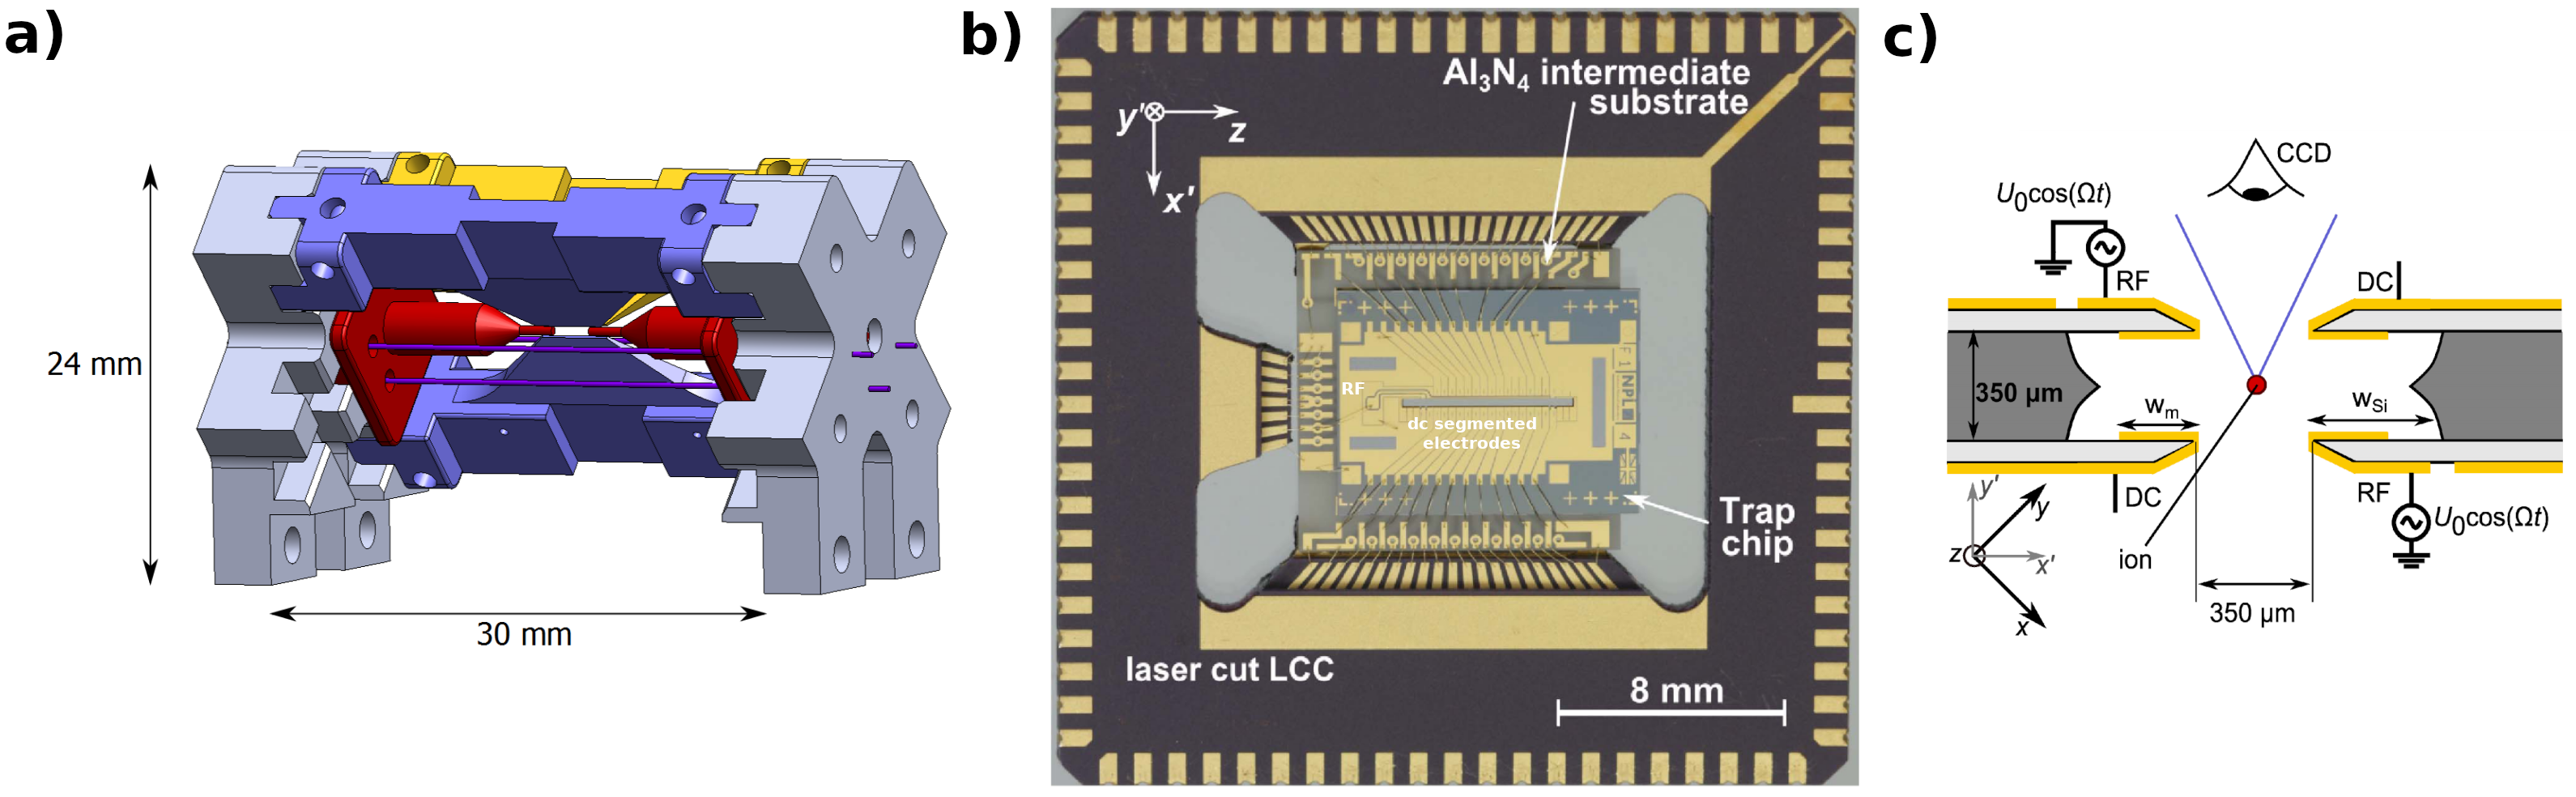
\includegraphics[width=\linewidth]{figures/png_figure/trap_comp.png}
        \end{center}
        \caption{\textbf{a)} XX Place holder figure. \textbf{b)} The NPL trap in use in this thesis. This is a microfabricated,
        segmented, multilayer trap. \textbf{c)} A cross sectional view of
        the NPL trap showing the RF and DC electrode positions.  Figures
        from~\cite{choonee_silicon_2017}.
        \label{fig:trap}}
    \end{figure}

    To create trapping potentials we use linear Paul traps, a schematic of such
    is shown in Figure~\ref{fig:trap}~(a). As explained by Earnshaw's theorem,
    $(\nabla^2 V = 0),$ a stable stationary point in 3D can not be realized
    using only static electric potentials, $V$, as if the potential is confining
    in two dimensions, it will be anticonfining in the third. Therefore, to
    achieve stable trapping either an oscillating electric field (Paul
    trap~\cite{XXX}), or a static magnetic field (Penning traps~\cite{XXX}) must
    be utilized to create a confining pseudopotential.\\
    Recently, the microfabricated surface style linear Paul trap has gained
    popularity due to the maturity of chip fabrication
    technologies~\cite{allcock_surface-electrode_2011} and the potential route
    to scalability this offers. In the surface trap, the 3D radial and axial
    electrodes of a ``macro'' trap are effectively projected onto a 2D surface.
    The stable point of such a trap is typically on the order of $50$ $\mu$m
    from the chip surface. The ease of fabrication of surface traps has allowed
    the creation of complex multizone devices with many DC electrodes.  These
    multizone traps enable the shuttling of ions, a requirement for Quantum CCD
    type architectures~\cite{kielpinski_architecture_2002}. However, this
    surface style geometry typically come with two costs: the depth of the
    trapping potential is often greatly reduced, and the close proximity of the
    surface to the ion can be a large contributor to motional heating
    rates~\cite{turchette_heating_2000}. \\
    The \emph{NPL} microfabricated 3D trap~\cite{see_fabrication_2013,
    wilpers_monolithic_2012}, as is used in our experiment, brings together the
    advantages of chip fabrication as well as the low heating rates and high
    trapping depths of a 3D style trap with greater ion-surface distances. This
    is achieved by a multilayer chip as shown in Figure~\ref{fig:trap}~(b, c).
    The radial trapping is provided by RF rails on opposite diagonals of the
    slit whilst axial trapping may be realized by the numerous DC electrodes.
    The ion-surface distance is now of the order $250$ $\mu$m and we have
    demonstrated heating rates of $ 33(3)$~q/s on a 4~MHz radial mode (see
    section~\ref{sec:Heating}).

    We aim for an axial ion separation of around $5$~$\mu$m which, for
    $^{40}$Ca$^{+}$ ions means a trapping potential of $\omega_z \approx 2\pi
    \cdot 1.6$~MHz. This ion separation was chosen to reduce the cross talk
    between ions when singly addressed (see section~\ref{sec:Single Addressing
    System}).\\ 
    We are targeting approximately $5$~MHz for our radial frequencies, as we
    shall use radial addressing for two-qubit entangling gates. The choice of
    this higher frequency is motivated by several factors. The Doppler cooling
    limit ($\overline{n} = \Gamma/\omega$, where $\Gamma$ is the transition
    linewidth and $\omega$ is the frequency of the cooled mode) inversely scales
    with the mode frequency. Consequently, higher mode frequencies result in
    lower temperatures following initial cooling. Additionally, a higher
    center-of-mass radial mode enables greater frequency separation of radial
    modes in a multi-ion crystal, which allow for greater selectivity of
    participating modes. \\ 
    Using the pseudopotential approximation~\cite{madsen_planar_2004} for the
    confining field, we can find a trapping frequency in one radial direction
    $\omega_p$
    \begin{equation}
    \omega_p = \frac{e\alpha V_{RF}}{\sqrt{2}\Omega_{RF}M\rho^2},
    \label{eq:pseudopotential}
    \end{equation}
    where $\alpha$ is a factor of order unity given by the geometry of the trap,
    $V_{RF}$ and $\Omega_{RF}$ are the voltage and frequency provided to the
    RF-electrode, $M$ is the mass of the ion, and $\rho$ is the ion-RF electrode
    separation.  Applying some DC voltage on the axial electrodes leads to axial
    confinement with frequency $\omega_{ax}$, but must defocus the radial
    confinements as the total curvature of the pseudopotential must remain
    constant,
    \begin{equation}
    \omega_{rad} = \sqrt{\omega_p^2 - \omega_{ax}^2/2}.
    \end{equation}
    Due to the geometry of the DC electrodes with respect to the ion chain, the
    \emph{NPL} trap focuses one of the radial modes and defocuses the other when
    the DC electrodes are increased,
    \begin{equation}
    \omega_{rad\pm} = \sqrt{\omega_p^2 - (1\mp\beta)\omega_{ax}^2/2},
    \end{equation}
    where $\beta$ is some factor due to the geometry of this geometry. From
    simulation $\beta > 1$ for $\Omega_{RF} = 2\pi\cdot 23$~MHz and $V_{RF} =
    200$~V and so one radial mode increases with DC voltage applied and one
    decreases.

    \begin{table}[h!]
    \begin{center}
    \begin{tabular}{ c|c c c c c }
    & $V_{RF}$/V &  $V_{DC}$/V &$\Omega_{RF}$/($2\pi\cdot$MHz)& $\omega$/($2\pi\cdot$MHz)   & q \\ 
    &  &  & & $\omega_{ax}$\quad   $\omega_{rad}$ &  \\ 
    \hline
    Experiment  & 200 & -7 &  23 & 1.6 \quad 4.9 & 0.61 \\
    Loading  & 100 & -2 &  23 & 0.8 \quad 2.0 & 0.25 \\
    \end{tabular}
    \caption{ Simulated trapping parameters for both ``Experiment'' and ``Loading'' settings \textsuperscript{40}Ca\textsuperscript{+} with the NPL trap. The ``Experiment'' setting is optimized for high axial mode frequencies whilst the ``Loading'' setting maintains a lower q factor for practical loading.  \label{table:freqs}}
    \end{center}
    \end{table}

    A possible set of parameters to achieve $\omega_{ax} = 2\pi \cdot 1.6$~MHz
    and $\omega_{rad+} = 2\pi \cdot 4.9$~MHz can be seen in the ``Experiment''
    trapping in Table~\ref{table:freqs}.

    From the Mathieu equations, the areas of stability depend upon a factor
    $q$~\cite{berkeland_minimization_1998}, where
    $q=2\sqrt(2)\omega/\Omega_{RF}$.  Generally, we require $q$ to be as low
    ($q<0.3$) for convenient trapping.  To satisfy this requirement a
    ``Loading'' setting (with parameters in table~\ref{table:freqs}) may be used
    with $q = 0.25$ and then the $V_{RF}$ ramped to the ``Experiment'' trapping
    for high radial mode frequencies.

\subsection{Trap RF Chain}
\label{sec:Trap RF Chain}
% Main points:
    % Maybe a figure describing the elements within the RF chain
        % Frequency source (Urukul)
        % Resonator
        % RF rails
    % Quote values we use.
% Pre reqs:
    % NPL trap geometry
    To utilise radial motional modes for low error quantum gates, we require the
    radio frequency (RF) field that produces the desired trapping
    pseudopotential to be both frequency and amplitude stable. Our \emph{NPL}
    trap is rated for a max peak-to-peak voltage of 400~Vpp on the RF
    electrodes. Here we describe the elements of the ``RF chain'' that supplies
    this voltage, as shown in figure~\ref{fig:RF Chain}. \\
    Our frequency source is a DDS-based synthesiser, named \emph{Urukul}, part
    of the \emph{Artiq Sinara}~\cite{XXX} hardware ecosystem. We operate the
    \emph{Urukul} at max output power, +10~dBm and with a frequency around $27.8$~MHz. This
    signal is then fed to an ``ultra-low noise limiting amplifier" named
    \emph{Squareatron}~\cite{XXX}. The purpose of \emph{Squareatron} is to
    greatly reduce the amplitude noise of the RF signal, $V_{\rm RF}$, which is
    key to low radial mode frequency drifts as can be seen by the linear
    relationship between trapping frequency and $V_{\rm RF}$ in
    equation~\ref{eq:pseudopotential}. The \emph{Squareatron} outputs +17.4~dBm,
    which we subsequently attenuate by 19.5~dB. We then amplify the signal by a
    further 33.7~dB using a \emph{Mini-Circuits ZHL-1-2W-S+}, high power
    amplifier. We now have +32 dBm RF power to drive the trap
    electrodes, however we need to match the current 50~$\Omega$ impedance to
    the small capacitance of the trap electrodes. To do this, we use an LC
    impedance matching circuit with tuned resonant frequency of 27.84~MHz, and a
    measured Q factor of 43.8 (found by fitting S11 impedance measurements).
    This resonant circuit has three main effects: it ensures good power transfer
    between RF input and trap electrodes via impedance matching, it steps up the
    voltage to the required 400~Vpp, and it filters out RF noise and unwated harmonics due to
    the narrow bandpass nature of the LC circuit. \\
    If components are chosen correctly, and adequately protected from
    environmental noise, this chain can produce the desired frequency and
    amplitude stable RF we require. Characterisations of the motional mode
    stability are discussed in section~\ref{sec:Motional Mode Stability}. We are
    still yet to fully quantify and debug the motional stability against thermal
    and mechanical noise, however it should be noted that other groups do opt
    for active stabilisation of RF amplitude through closed feedback loops~\cite{XXX}.\\
    % Milne sydney trap RF chain 

%\subsection{Trap DC Voltages}
% Main points:
    % Describe Fastino DAC and the available electrodes on the NPL trap
    % Quote values we use.
% Pre reqs:
    % NPL trap geometry

\section{Magnetic Field}
\label{sec:Magnetic Field}
% Main points:
    % Permanent magnets
    % MUMetal box
    Stable Zeeman shifts of the ion energy levels are required for long spin
    coherence times (see section~\ref{sec:Coherence}), and for low error single
    and two qubit gates. We use a permanent magnet array of Samarium Cobalt,
    Sm$_2$Co$_17$, in a Helmholtz configuration to create a stable magnetic
    field of 5.4~G. Samarium Cobalt was chosen for its low temperature
    coefficient of remenance, -0.03\%/K.\\
    The ion is shielded from unwanted external magnetic fields by two layers of
    3~mm thick MuMetal shielding from \emph{MagneticShields}. The factory quoted
    shielding factor is 546 for DC fields. Spin coherence time comparisons for
    the ion with and without magnetic shielding are shown in
    section~\ref{sec:Coherence}.\\

\section{Vacuum System and Beam Geometry}
\label{sec:Vacuum System}
% Main points:
    % Technical drawing of beam geometries and magnetic field to ion chain.
    % Drawing of ion trap package with high NA lenses
        % High NA sandwich
    % Standing waves at the ion
% Pre reqs:
    % NPL trap
    % Why we have Dual high NA lenses
    % Magnetic field giving Zeeman shift


\begin{figure}
  \begin{center}
   \noindent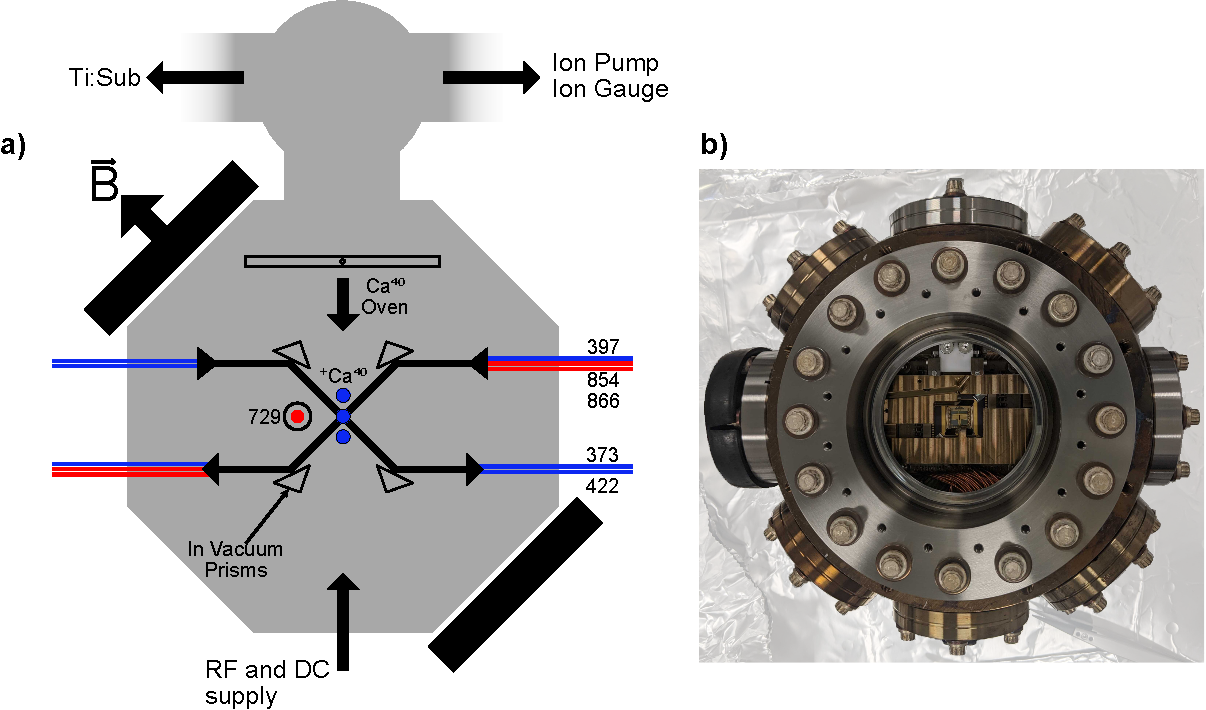
\includegraphics[width=0.9\linewidth]{figures/pdf_figure/vacuum_can-crop.pdf}
  \end{center}
  \caption{
    \textbf{a)} XXX Place holder figure. A schematic of the vacuum chamber.
    Wavelengths apart from 729-nm enter through the side CF40 viewports and are
    directed onto the ions by in vacuum prisms. The 729-nm light enters through
    the larger CF100 viewports.  \textbf{b)} A photograph of the assembled
    system prior to baking.
  }
  \label{fig:can}
\end{figure}


\begin{figure}
  \begin{center}
   \noindent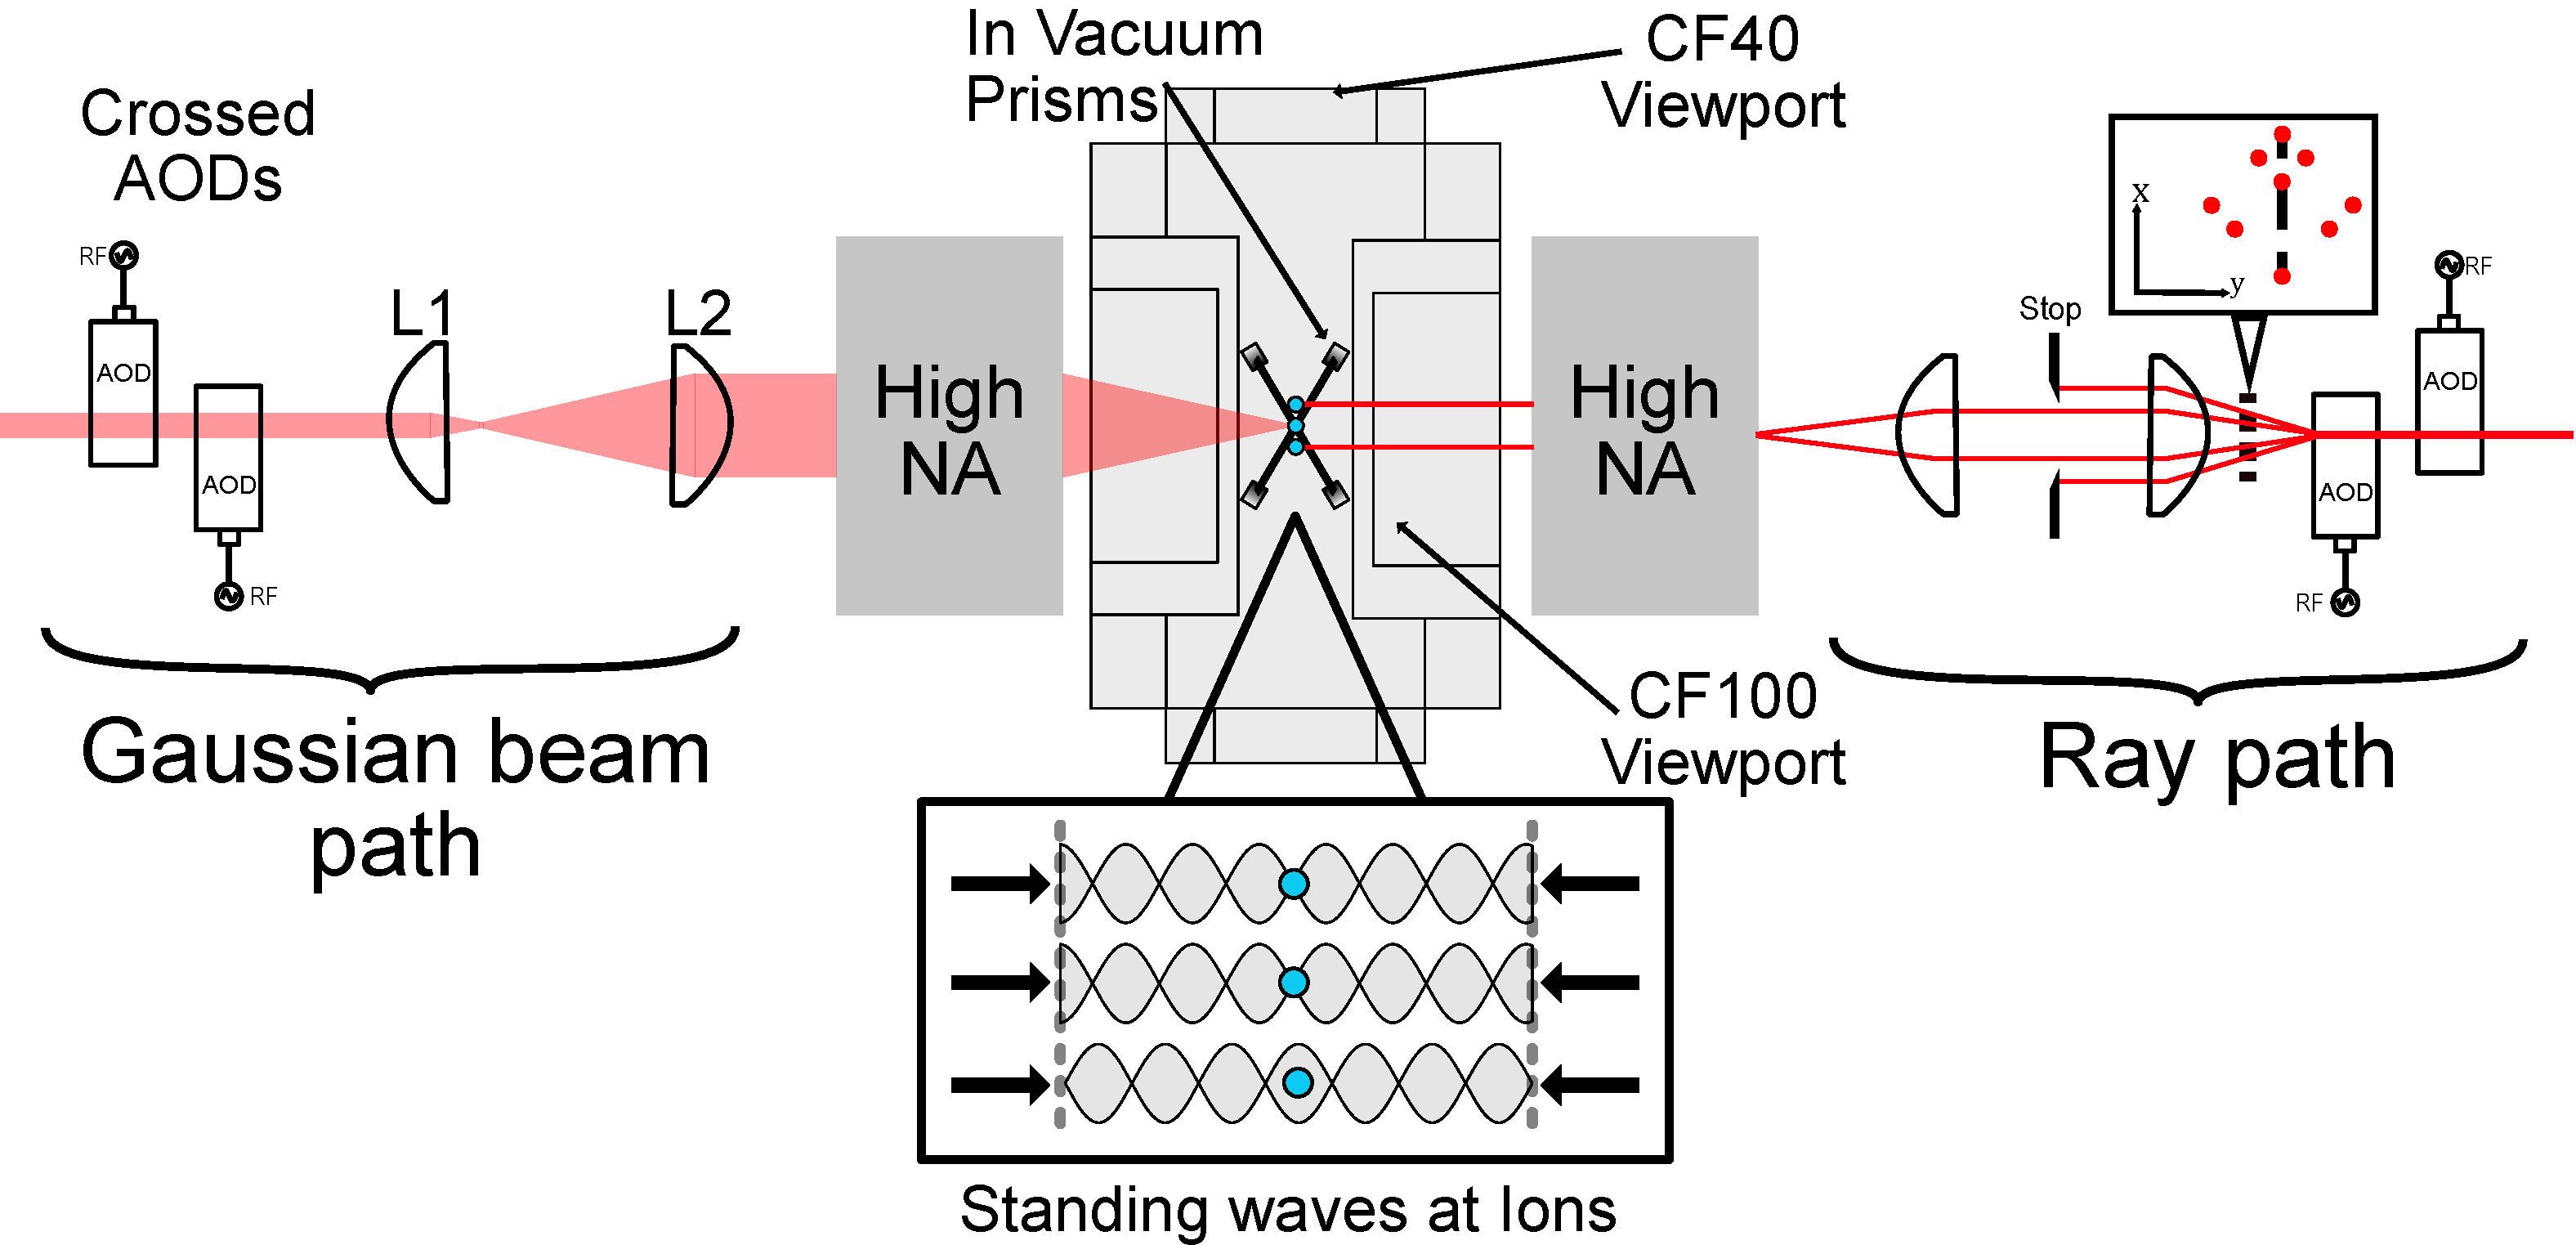
\includegraphics[width=\linewidth]{figures/pdf_figure/vac_can_AOD_small.pdf}
  \end{center}
  \caption{XXX Place holder figure. The standing wave single addressing system. Dual high NA
    objectives focus the light to a tight waist at the ions
    location. AODs are used to steer the light to only selected
    ions. The left hand side of the figure shows the Gaussian profile
    of the light, whilst the right hand side shows a ray
    representation of how two singly addressing spots are formed at
    the ions. L1 is a telecentric scanning lens and in combination
    with L2 form a beam expander.}
  \label{fig:AOD}
\end{figure}

    Ultra High Vacuum (UHV) is required to extend the ion storage lifetime.
    However, UHV equipment is often bulky, and puts constraints on the access
    and visibility of the ion chain. Here we describe the designed vacuum
    system, and beam access.  The vacuum system and beam geometries were
    designed by Sebastian Saner and Mariella Minder, and constructed by
    Sebastian Saner, Fabian Pokorny, and myself.\\
    
    We aim for a residual pressure of $<10^{-11}$ mbar. For this strict
    requirement, we must take care in selecting in-vacuum materials, and follow
    thorough cleaning and baking procedures. A summary of tactics that were
    useful in the construction of the vacuum system can be found
    in~\cite{birnbaum_ultra-high_2005, wolf_cryogenic_2019}.\\
    A schematic and photograph of the vacuum system can be seen in
    Figure~\ref{fig:can}. The system consists of a 6" spherical-octagonal
    experimental chamber\footnote{Kimball MCF600-SphOct-F2C8} connected to a
    spherical chamber with ion pump\footnote{Agilent VacIon Plus 20 Pump}, ion
    gauge\footnote{Agilent UHV-24P Ion gauge} and Titanium sublimator pump
    (TSP)\footnote{Scanwel custom housing} attached. The ion pump and TSP
    maintain the UHV to the desired $<10^{-11}$~mbar. We find that on the ion
    pump alone we cannot maintain UHV indefinitely, however, firing the TSP
    every 4 weeks with 41~A for 60 seconds provides a sufficient pumping rate.
    At the time of system baking, we performed a He leak test, but did not find
    any external leaks. We suspect the gradual pressure increase is either due
    to our use of in-vacuum optics, optics epoxy adhesive\footnote{EPO-TEK
    353ND}, or our use of soldered PCB components.\\
    For optical access we have two recessed CF100 viewports\footnote{UK Atomic
    Energy Authority P/N VPR100015} on the two large faces of the experiment
    can. We require recessed viewports due to our chosen main
    objectives\footnote{Photon Gear custom Atom Imager}. These custom objectives
    have an effective focal length of 33~mm, a working distance of 24.4~mm, and
    a numerical aperture of 0.6. They are coated for 397-nm and 729-nm.
    The consideration for dual high NA objectives is relatively unique in ion trap experiments, and was mainly motivated by previous work on fast entangling gates via standing waves~\cite{saner_breaking_2023}. \\
    There is further optical access via
    two CF40 side viewports\footnote{LewVac ZFSVP-DUV-40CF-OUM} coated
    for 397-nm, 422-nm, 729-nm, 854-nm and 866-nm.  Due to the spatial
    constraints from the trap assembly and high NA objectives, we require
    multiple of our beam to enter the vacuum can through these side ports. For the ion chain to be visible from these side ports we use in vacuum dielectric
    mirrors. These fused-silica mirrors are UHV rated and coated for 372-nm, 397-nm,
    422-nm, 729-nm, 854-nm and 866-nm, with reflectivities of >99\% for both s-
    and p-polarised light. Figure~\ref{fig:can} shows a schematic of the beam
    geometries via the side ports. A limitation of this beam geometry is that due to the permanent B-field direction, we are unable to apply pure $\pi$ or $\sigma_{\pm}$ light to the ion. However for applications where strict polarisation control is needed, the beams can be incident through the CF100 viewport.\\
    We use an electrical feedthrough on a CF40 flange\footnote{Allectra custom}
    to supply our trap chip and atomic source oven with DC and RF voltages. As
    the DC cables run within close proximity to the RF supply, electrical pick
    up is a potential issue for our DC lines. RF leaked onto our DC electrodes
    will create unwanted pseudopotential which can lead to unexpected mode
    geometries, or required compensation field. We mitigate this leakage through
    an in-vacuum RC low pass filter board within close proximity of the trap
    chip with a cutoff frequency of 17~kHz. The trap chip is mounted onto this
    filter board via a custom Polyether ether ketone (PEEK) interposer with
    electric feedthroughs via embedded \emph{Fuzz buttons}\footnote{Custom
    Interconnects}. \\

\section{Ca$^+$ Laser Systems}	
\label{sec:Laser systems}
% Main points:
    % State which lasers we need access to
    % Calcium level structure 
    % What frequency control do we need on each? PDH lock, AOM etc.
    % Table of all AOMs and offset frequencies
    % Table of laser powers in mW and with aimed saturation intensities for doppler idle, cooling, readout, and laser linewidths.
% Pre reqs:
    % Calcium level structure
    % 5 G field
    \begin{figure}[ht]
        \begin{center}
        \noindent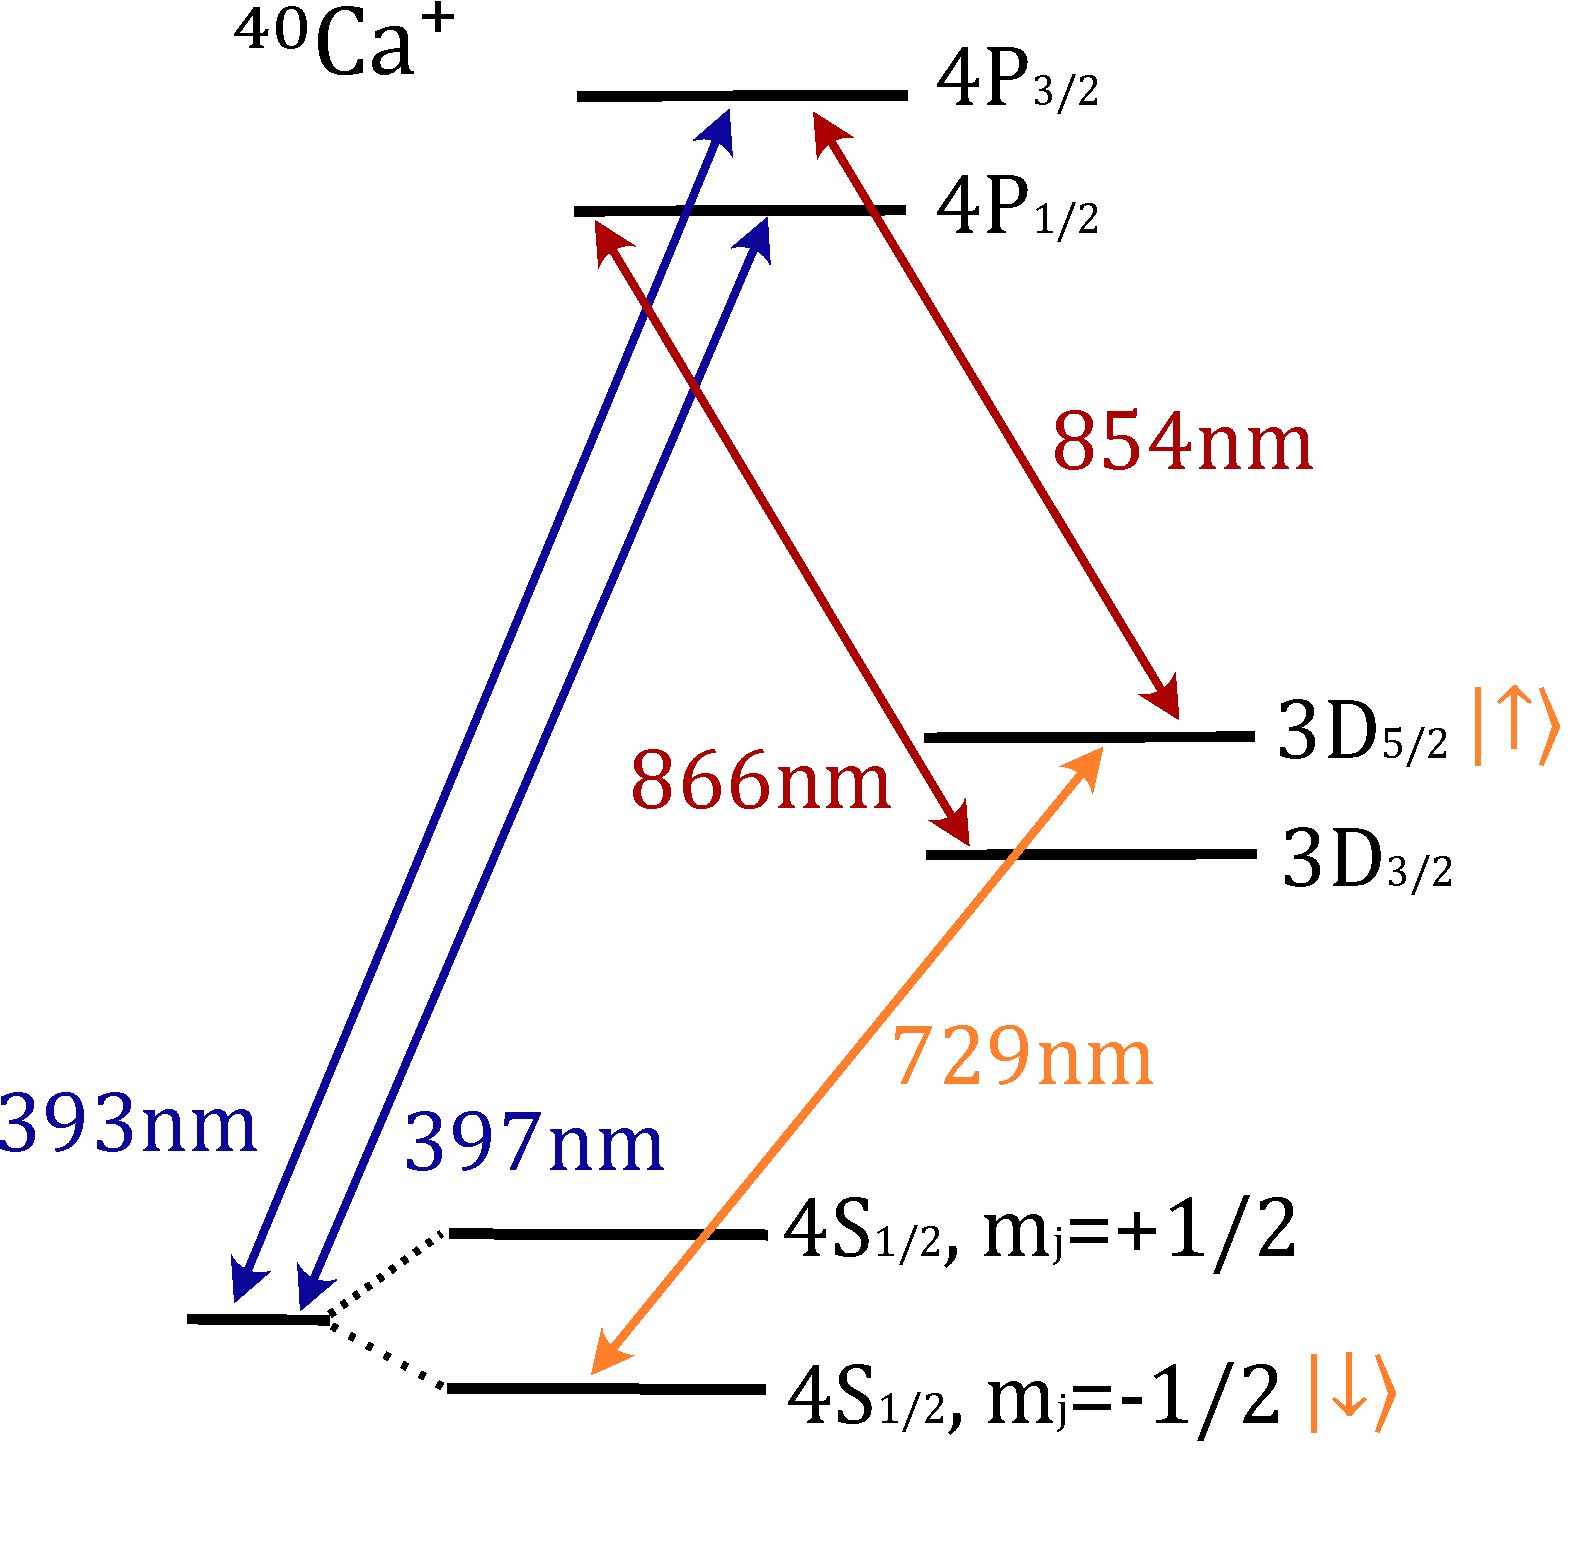
\includegraphics[width=0.4\linewidth]{figures/pdf_figure/Ca40.pdf}
        \end{center}
        \caption{
        Electronic energy levels of \textsuperscript{40}Ca\textsuperscript{+},
        which will be used in this thesis. The levels are
        split by the Zeeman effect due to a $5.4$~G external magnetic field (they are shown explicitely only for the ground state). The
        transitions marked are required for cooling and control over the
        ion. We shall use the optical-qubit with a quadrupole transition at
        729-nm. XXX TODO: Add zeeman levels for D5/2.
        }

    \label{fig:ion}
    \end{figure}

    Singly-charged group 2 elements are popular in ion trap
    experiments due to their single outer electron resulting in Hydrogen-like
    energy levels. In this thesis we use \ca.\\
    \ca has
    no nuclear spin giving the
    (relatively) simple level structure shown in figure~\ref{fig:ion}. The external
    magnetic field of $5.4$~G is applied to split the levels via the Zeeman
    effect. The relevant laser transitions for our planned ion trap
    experiment are indicated.\\
    A zero nuclear spin isotope of calcium was chosen due to this simple level
    structure without hyperfine splitting. The greater number of levels due to
    hyperfine splitting lead to more decay paths and therefore greater
    complications in both cooling and gate schemes. However, this does come at
    the cost of no available magnetic field insensitive transitions, which are
    often used in ion trap experiments to further decouple the ion from a noisy
    environment~\cite{}. \\
    We define our qubit by the quadrupole transition at 729-nm, which we describe in the following section.\\
    Access to other excited levels, outside of our defined two level system, are crucial for ion trap quantum logic so that we can readout the qubit with state selective fluorescence (397-nm, and 866-nm transitions) and optically pump for state preparation (397-nm, 866-nm, and 854-nm transitions). Details on these schemes are given in chapter~\ref{ch:Characterisation}. We also require access to two additional transitions in neutral calcium for isotope selective ionisation, 422-nm and 372-nm.\\
    These transitions (apart from the 729-nm) are all driven by diode lasers\footnote{All Toptica diodes. Red lasers: MDL DL pro; Blue lasers: MDL DL pro HP; 372-nm: iBEAM-SMART-375-S}, which are frequency stabilised to a reference cavity\footnote{Stable Laser Systems SLS-6010 4-Bore Cylindrical Cavity} via Pound-Drever-Hall (PDH) locking. We require PDH locking to ensure that laser frequencies are stable to <1~MHz level, well below the natural line widths of all the dipole transitions listed above. We continuosly monitor the laser frequencies with a wavemeter\footnote{HighFinesse WS7}.\\
    Frequency and amplitude control for all lasers is achieved via acousto-optic modulators (AOMs) which are driven by Artiq integrated DDS chips, \emph{Urukuls}. We use AOMs in a double pass configuration to allow shifts of the laser frequency by +/- ~100~MHz, with no signicant angular shifts or loss of fibre coupling. 
    
    
\subsection{Narrow Line Width 729 Laser}
\label{sec:Narrow Line Width 729 Laser} 
% Main points:
    % What equipment does the 729 consist of.
    % Solstis cavity
    % Beam path and control loops (PDH, FNC)
    % Frequency shifting, pulse carving via urukul
    % Amplitude stabilisation with SUServo
% Pre reqs:
    % Calcium level structure

    Lasers are a key tool for creating the highly localised, strong electric
    field amplitudes and gradients needed to drive both carrier and sideband
    transitions of the trapped ion.\\ As shown in Figure~\ref{fig:ion}, we will
    use two levels within the 4S\textsubscript{1/2} to 3D\textsubscript{5/2}
    manifolds to define our qubit. This is an electric quadrupole transition as
    $\Delta l = 2$.  For the Calcium ion this transition is at 729-nm, and so we
    use a near resonance 729-nm laser to implement single- and multi-qubit gates
    (sections~\ref{sec:Randomised Benchmarking} and~\ref{sec:Two-Qubit
    Entangling Gates}). We also use this transition, after Doppler cooling, for
    resolved sideband cooling to bring the motional mode close to its ground
    state (as discussed in section~\ref{sec:Cooling}).

    This transition is narrrow line width due the the long lived
    3D\textsubscript{5/2} state, and so, for power efficiency, we must use a
    narrow linewidth laser. For our ``fast entangling gates'' use case we
    require large electric-field intensities at the ion to drive sideband
    transitions, this will be discussed further in the single-addressing and
    two-qubit gate sections, but here it is sufficient to say we require >100 mW
    of light at the ion plane.  Here we describe the built system 
    consisting of a Ti:Sapph laser system pumped with by an Nd:YAG 532-nm laser.\\

    We pump an \emph{M2 Solstis} Ti:Sapph~\cite{XXX} with 18 W of 532-nm light
    from a \emph{Coherent Verdi-V} system~\cite{XXX} to produce around 5W of
    729-nm light.  The Ti:Sapph is engineered to operate with a stable $<50$~kHz
    linewidth. Ti:Sapph crystals have broadband gain profiles~\cite{XXX}, which
    is often exploited in research environments to create frequency tunable
    laser systems. We however want a narrow linewidth, single frequency laser,
    and so the \emph{Solstis} has multiple intracavity frequency selective
    elements. These consist of (in order of coarse frequency selectivity), a
    birefringent filter, a tunable Fabry-P\'erot etalon, and the surrounding
    bow-tie cavity. For stable single mode operation, the \emph{Solstis} employs
    an active ``dither" servo to lock the peak of etalon transmission to one of
    the cavity longitudinal mode. This dither consists of periodically varying
    the etalon spacing with a frequency of around 20~kHz. We must be aware of
    this dither frequency as the phase modulation leads to the creation of
    sidebands on our light which can interact with the ion causing unexpected
    errors in gates. We can observe this dither frequency (and harmonics of it)
    with our ion via composite pulse experiments, however it is currently not
    expected to be a limiting source of error in any of our desired interactions
    we study.\\
    \begin{figure}
    \begin{center}
    \noindent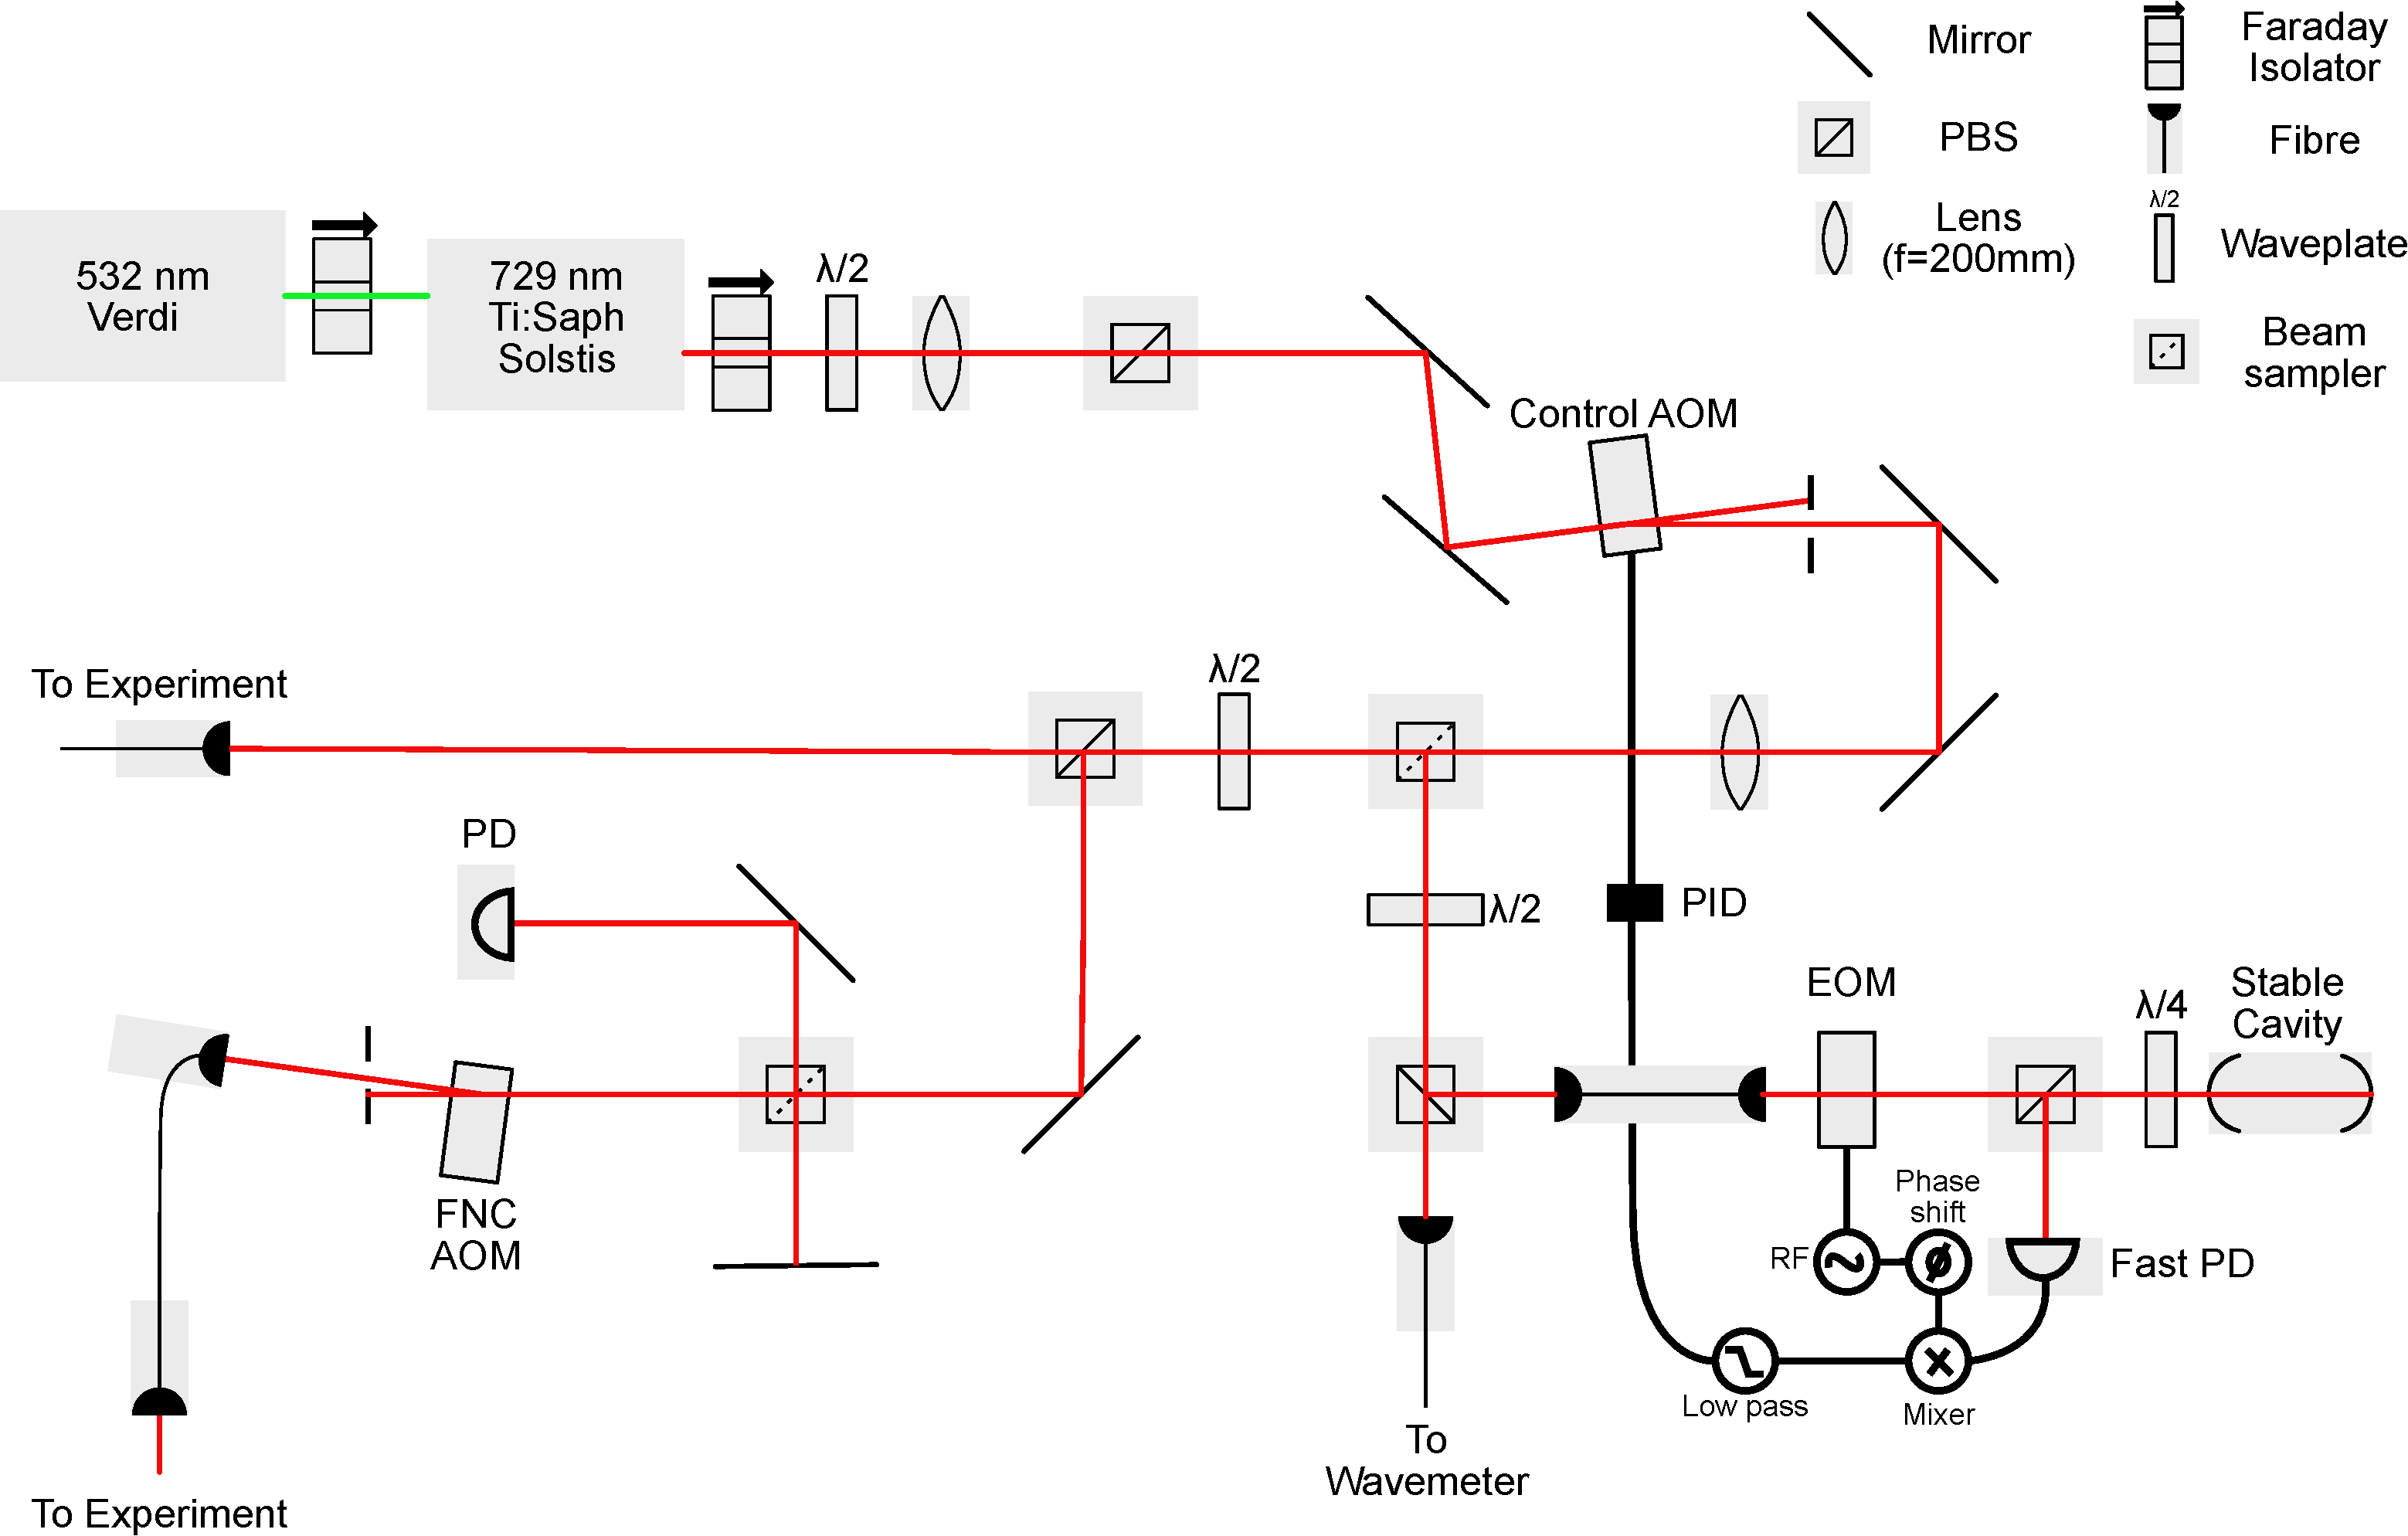
\includegraphics[width=0.9\linewidth]{figures/pdf_figure/729_path_small.pdf}
    \end{center}
    \caption{The 729-nm system. A Ti:Sapph laser tuned to 729-nm is
        pumped by a 532-nm source. Light is picked off at the first beam
        sampler to stabilise by PDH locking to a cavity.}
    \label{fig:729}
    \end{figure}
    \begin{figure}
        \begin{center}
        \noindent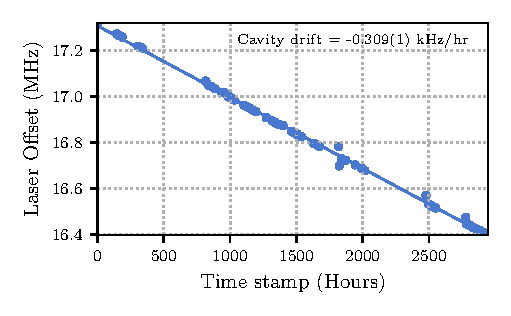
\includegraphics[width=0.75\linewidth]{
            figures/pdf_figure/cavity_drift.pdf
            }
        \end{center}
        \caption{
            Cavity drift over 125 days. Extracted by reference to ion transition.
            }
        \label{fig:Cavity Drift}
    \end{figure}
    As mentioned, the \emph{Solstis} alone can operate with linewidths of
    $<50kHz$, however we push this further by referencing the Ti:Sapph output
    with an ulta high finesse cavity by \emph{Stable Laser Systems} and applying
    a Pound-Drever-Hall (PDH) lock~\cite{}.  A schematic of our 729-nm system is
    shown in Figure~\ref{fig:729}.  PDH locking requires applying two sidebands
    via an electro-optical modulator (EOM) to the light and directing it onto
    the stable cavity. The light reflected from the cavity is then directed onto
    a fast photodetector (\emph{Thorlabs PDA10A2}). The reflection from the
    cavity consists of the interference between the carrier and the sidebands
    which have been respectively altered by the cavity transfer function. The
    photodetector signal is mixed down with the same oscillator signal as
    provided to the EOM but delayed by some chosen phase, and finally low pass
    filtered to produce a signal for use as the error signal in the servo loop.
    This error gives a measure for how far the carrier frequency is from the
    stable cavity resonant frequency and is used for feedback onto the control
    AOM situated after the Solstis. The electronics for this control loop are
    provided also by Stable Laser Systems in the form of their \emph{FPGA Servo}
    lock box. For an effective PDH lock, we require both short and long term
    stability of our reference cavity. To ensure the cavity is insensitive to
    the environment, it is made of an ultra low expansion material. We
    temperature stabilise the cavity at the zero crossing temperature of
    $30.6^\circ$C, and it is further isolated by being stored in a vacuum system
    at $<1e-7$~mbar. We measure a long term cavity drift of 309(1) Hz/hr over
    125 days, seen in figure~\ref{fig:729}. This measurement uses the ion as a
    frequency reference to probe the cavity frequency and is discussed in
    section~\ref{sec:Laser Offset}.\\
    Figure~\ref{fig:729} displays the other beam paths for our 729-nm system.
    Some light is picked off and sent to a wavemeter to continuosly monitor the
    frequency. However, the majority is coupled to two output fibres for our
    experiment and another within the group. We transport the 729-nm light from
    a dedicated laser lab to a room containing the trap apparatus by a 10~m
    single mode polarization maintaining fibre (\emph{SKXXX}).  The fibre is
    beneficial in cleaning up the mode from the Ti:Sapph, however it can
    introduce phase noise due to mechanical and thermal effects along the 10~m
    length. To remove this introduced noise we utilise passive stabilisation in
    the form of thick foam tubing along the fibre length as well as active
    stabilisation by popular fibre-noise-cancellation technique~\cite{XXX}. This
    topic has been discussed extensively in multiple PhD and Masters
    theses~\cite{XXX}, and so here we only quote the relevant control aspects of
    our arrangement. We use the \emph{Sinara Stabilizer}~\cite{XXX} board, a
    dual channel PID microcontroller, with the \emph{Pounder}~\cite{XXX}
    mezzanine board, a dual channel PDH lock generator. The FNC PID software was
    developed by Ayush Agrawal ~\cite{XXX}. A comparison of spin coherence times
    is shown in section~\ref{sec:Coherence} with and without fibre noise
    cancellation enabled. \\


\subsection{Single Addressing System}
\label{sec:Single Addressing System}
% This section is not used in any characterisation - could be left for outlook!
% Main points:
    % The advantages of single addressing using AODs
        % Ion selectivity
        % High intensity electric field
    % single addressing system creating standing waves
    % render of single addressing system
% Pre reqs:
    % 729 system
    % High NA
    % Trap package
    % Motivation for future experiments
    A unique feature of our system is the ability to produce standing wave
    single ion addressing. The design of this system is shown in
    figure~\ref{fig:AOD}.  A single ion addressing system must be able to
    illuminate selected ions in the crystal whilst the others remain
    unperturbed. The advantage of single addressing, other than ion selectivity,
    is the increased intensity of light due to the tight waist at the ion
    location. \\
    Our ions will be separated by a distance $d\approx 5~\mu$m.  Focussing a
    collimated 729-nm beam with an objective lens of NA = 0.6 onto the ion
    provides $\omega_0 = 386$~nm.  Abberations present in real optical
    components will cause the addressed spot to be increasingly non-gaussian and
    lead to unfavourable cross talk at the neighbouring ions. Therefore care is
    taken in the optical design.\\
    To produce more than one addressed spot and to steer the spots along the ion
    crystal, we use Acousto-Optical-Deflectors\footnote{ISOMET OAD1343-XY-T70S}
    (AODs)~\cite{nagourney_quantum_2014, li_low-crosstalk_2023,
    pogorelov_compact_2021}. The beam deflection angle is proportional to the
    drive frequency supplied to the AOD. \\


%%%%% REFERENCES

\setlength{\baselineskip}{0pt} % JEM: Single-space References

{\renewcommand*\MakeUppercase[1]{#1}%
\printbibliography[heading=bibintoc,title={\bibtitle}]}


\end{document}